\appendix
\chapter{Befehlsliste}
\label{a:befehlsliste}
\section*{\textit{Erklärungen}}
Alle Befehle, die mit \textbf{.u} (engl. \textit{unsigned}) enden, werden als
vorzeichenunbehaftet betrachtet und alle Befehle, die mit \textbf{.s}
(engl. \textit{signed}) enden, werden als vorzeichenbehaftet betrachet.

Wenn ein Befehl auf Vorzeichen achtet und dies nicht angegeben
wird (also kein \textbf{.u} oder \textbf{.s}), ist der Befehl äquivalent zum
vorzeichenunbehafteten Befehl, wenn es nicht explizit angegeben wird.
\section*{nop}
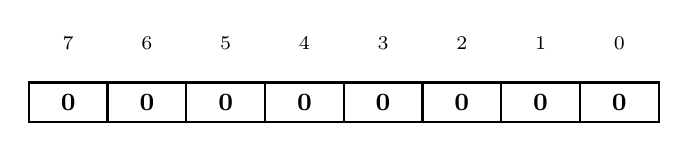
\begin{tikzpicture}
	% Bitnummern oben
	\foreach \x in {0,...,7}
		\pgfmathsetmacro{\number}{int(abs(\x-7))}
		\node at (\x - 0.5, 20.5) {\scriptsize \number};
	% Bitbeschreibungen
	\filldraw[thick, draw=black, fill={rgb:white,255}] (-1, 20) rectangle (0,
	19.5);
	\node (mode) at (-0.5, 19.75) {\small \textbf{0}};
	\filldraw[thick, draw=black, fill={rgb:white,255}] (0, 20) rectangle (1,
	19.5);
	\node (mode) at (0.5, 19.75) {\small \textbf{0}};
	\filldraw[thick, draw=black, fill={rgb:white,255}] (1, 20) rectangle (2,
	19.5);
	\node (mode) at (1.5, 19.75) {\small \textbf{0}};
	\filldraw[thick, draw=black, fill={rgb:white,255}] (2, 20) rectangle (3,
	19.5);
	\node (mode) at (2.5, 19.75) {\small \textbf{0}};
	\filldraw[thick, draw=black, fill={rgb:white,255}] (3, 20) rectangle (4,
	19.5);
	\node (mode) at (3.5, 19.75) {\small \textbf{0}};
	\filldraw[thick, draw=black, fill={rgb:white,255}] (4, 20) rectangle (5,
	19.5);
	\node (mode) at (4.5, 19.75) {\small \textbf{0}};
	\filldraw[thick, draw=black, fill={rgb:white,255}] (5, 20) rectangle (6,
	19.5);
	\node (mode) at (5.5, 19.75) {\small \textbf{0}};
	\filldraw[thick, draw=black, fill={rgb:white,255}] (6, 20) rectangle (7,
	19.5);
	\node (mode) at (6.5, 19.75) {\small \textbf{0}};
\end{tikzpicture}

Dieser Befehl führt keine Operation aus.
\section*{add.u, add.s}
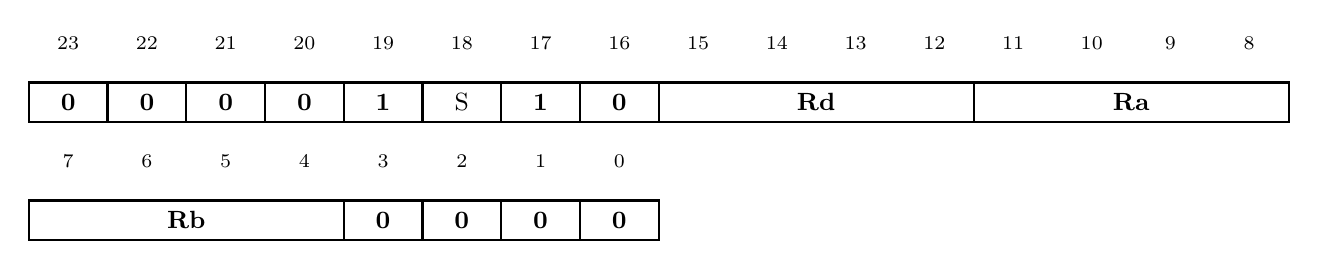
\begin{tikzpicture}
	% Bitnummern oben
	\foreach \x in {0,...,15}
		\pgfmathsetmacro{\number}{int(abs(\x-15)+8)}
		\node at (\x - 0.5, 20.5) {\scriptsize \number};
	% Bitbeschreibungen
	\filldraw[thick, draw=black, fill={rgb:white,255}] (-1, 20) rectangle (0,
	19.5);
	\node (mode) at (-0.5, 19.75) {\small \textbf{0}};
	\filldraw[thick, draw=black, fill={rgb:white,255}] (0, 20) rectangle (1,
	19.5);
	\node (mode) at (0.5, 19.75) {\small \textbf{0}};
	\filldraw[thick, draw=black, fill={rgb:white,255}] (1, 20) rectangle (2,
	19.5);
	\node (mode) at (1.5, 19.75) {\small \textbf{0}};
	\filldraw[thick, draw=black, fill={rgb:white,255}] (2, 20) rectangle (3,
	19.5);
	\node (mode) at (2.5, 19.75) {\small \textbf{0}};
	\filldraw[thick, draw=black, fill={rgb:white,255}] (3, 20) rectangle (4,
	19.5);
	\node (mode) at (3.5, 19.75) {\small \textbf{1}};
	\filldraw[thick, draw=black, fill={rgb:white,255}] (4, 20) rectangle (5,
	19.5);
	\node (mode) at (4.5, 19.75) {\small S};
	\filldraw[thick, draw=black, fill={rgb:white,255}] (5, 20) rectangle (6,
	19.5);
	\node (mode) at (5.5, 19.75) {\small \textbf{1}};
	\filldraw[thick, draw=black, fill={rgb:white,255}] (6, 20) rectangle (7,
	19.5);
	\node (mode) at (6.5, 19.75) {\small \textbf{0}};
	\filldraw[thick, draw=black, fill={rgb:white,255}] (7, 20) rectangle (11,
	19.5);
	\node (mode) at (9, 19.75) {\small \textbf{Rd}};
	\filldraw[thick, draw=black, fill={rgb:white,255}] (11, 20) rectangle (15,
	19.5);
	\node (mode) at (13, 19.75) {\small \textbf{Ra}};

	% Bitnummern oben
	\foreach \x in {0,...,7}
		\pgfmathsetmacro{\number}{int(abs(\x-7))}
		\node at (\x - 0.5, 19) {\scriptsize \number};
	% Bitbeschreibungen
	\filldraw[thick, draw=black, fill={rgb:white,255}] (-1, 18.5) rectangle (3,
	18);
	\node (mode) at (1, 18.25) {\small \textbf{Rb}};
	\filldraw[thick, draw=black, fill={rgb:white,255}] (3, 18.5) rectangle (4,
	18);
	\node (mode) at (3.5, 18.25) {\small \textbf{0}};
	\filldraw[thick, draw=black, fill={rgb:white,255}] (4, 18.5) rectangle (5,
	18);
	\node (mode) at (4.5, 18.25) {\small \textbf{0}};
	\filldraw[thick, draw=black, fill={rgb:white,255}] (5, 18.5) rectangle (6,
	18);
	\node (mode) at (5.5, 18.25) {\small \textbf{0}};
	\filldraw[thick, draw=black, fill={rgb:white,255}] (6, 18.5) rectangle (7,
	18);
	\node (mode) at (6.5, 18.25) {\small \textbf{0}};
\end{tikzpicture}

Addiere zwei Register miteinander. Das Bit \textbf{S} zeigt an, ob die Addition
vorzeichenbehaftet(1) oder vorzeichenunbehaftet(0) stattfinden soll.

\textit{Regs[Rd] = Regs[Ra] + Regs[Rb]}
\section*{addi.u, addi.s}
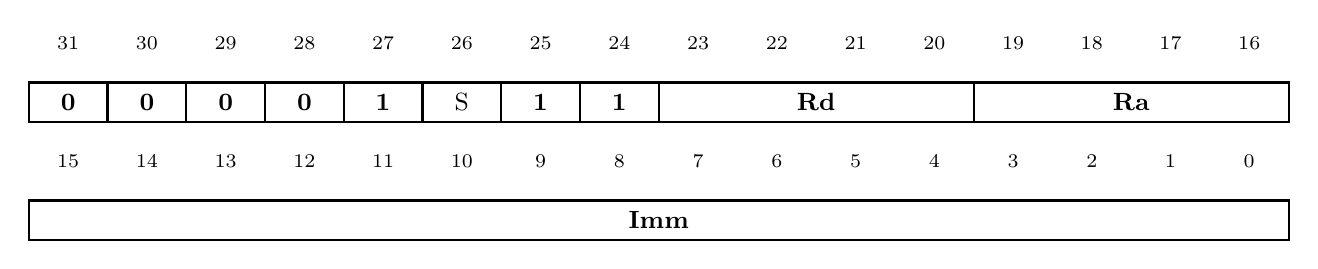
\begin{tikzpicture}
	% Bitnummern oben
	\foreach \x in {0,...,15}
		\pgfmathsetmacro{\number}{int(abs(\x-15)+16)}
		\node at (\x - 0.5, 20.5) {\scriptsize \number};
	% Bitbeschreibungen
	\filldraw[thick, draw=black, fill={rgb:white,255}] (-1, 20) rectangle (0,
	19.5);
	\node (mode) at (-0.5, 19.75) {\small \textbf{0}};
	\filldraw[thick, draw=black, fill={rgb:white,255}] (0, 20) rectangle (1,
	19.5);
	\node (mode) at (0.5, 19.75) {\small \textbf{0}};
	\filldraw[thick, draw=black, fill={rgb:white,255}] (1, 20) rectangle (2,
	19.5);
	\node (mode) at (1.5, 19.75) {\small \textbf{0}};
	\filldraw[thick, draw=black, fill={rgb:white,255}] (2, 20) rectangle (3,
	19.5);
	\node (mode) at (2.5, 19.75) {\small \textbf{0}};
	\filldraw[thick, draw=black, fill={rgb:white,255}] (3, 20) rectangle (4,
	19.5);
	\node (mode) at (3.5, 19.75) {\small \textbf{1}};
	\filldraw[thick, draw=black, fill={rgb:white,255}] (4, 20) rectangle (5,
	19.5);
	\node (mode) at (4.5, 19.75) {\small S};
	\filldraw[thick, draw=black, fill={rgb:white,255}] (5, 20) rectangle (6,
	19.5);
	\node (mode) at (5.5, 19.75) {\small \textbf{1}};
	\filldraw[thick, draw=black, fill={rgb:white,255}] (6, 20) rectangle (7,
	19.5);
	\node (mode) at (6.5, 19.75) {\small \textbf{1}};
	\filldraw[thick, draw=black, fill={rgb:white,255}] (7, 20) rectangle (11,
	19.5);
	\node (mode) at (9, 19.75) {\small \textbf{Rd}};
	\filldraw[thick, draw=black, fill={rgb:white,255}] (11, 20) rectangle (15,
	19.5);
	\node (mode) at (13, 19.75) {\small \textbf{Ra}};

	% Bitnummern oben
	\foreach \x in {0,...,15}
		\pgfmathsetmacro{\number}{int(abs(\x-15))}
		\node at (\x - 0.5, 19) {\scriptsize \number};
	% Bitbeschreibungen
	\filldraw[thick, draw=black, fill={rgb:white,255}] (-1, 18.5) rectangle (15,
	18);
	\node (mode) at (7, 18.25) {\small \textbf{Imm}};
\end{tikzpicture}

Addiere ein Register mit einer 16-Bit-Konstanten. Das Bit \textbf{S} zeigt an,
ob die Addition vorzeichenbehaftet(1) oder vorzeichenunbehaftet(0) stattfinden
soll.

\textit{Regs[Rd] = Regs[Ra] + Imm}
\section*{sub.u, sub.s}
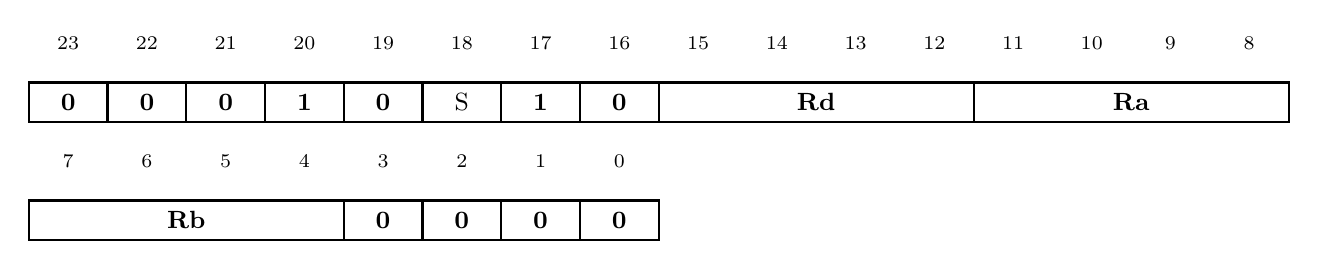
\begin{tikzpicture}
	% Bitnummern oben
	\foreach \x in {0,...,15}
		\pgfmathsetmacro{\number}{int(abs(\x-15)+8)}
		\node at (\x - 0.5, 20.5) {\scriptsize \number};
	% Bitbeschreibungen
	\filldraw[thick, draw=black, fill={rgb:white,255}] (-1, 20) rectangle (0,
	19.5);
	\node (mode) at (-0.5, 19.75) {\small \textbf{0}};
	\filldraw[thick, draw=black, fill={rgb:white,255}] (0, 20) rectangle (1,
	19.5);
	\node (mode) at (0.5, 19.75) {\small \textbf{0}};
	\filldraw[thick, draw=black, fill={rgb:white,255}] (1, 20) rectangle (2,
	19.5);
	\node (mode) at (1.5, 19.75) {\small \textbf{0}};
	\filldraw[thick, draw=black, fill={rgb:white,255}] (2, 20) rectangle (3,
	19.5);
	\node (mode) at (2.5, 19.75) {\small \textbf{1}};
	\filldraw[thick, draw=black, fill={rgb:white,255}] (3, 20) rectangle (4,
	19.5);
	\node (mode) at (3.5, 19.75) {\small \textbf{0}};
	\filldraw[thick, draw=black, fill={rgb:white,255}] (4, 20) rectangle (5,
	19.5);
	\node (mode) at (4.5, 19.75) {\small S};
	\filldraw[thick, draw=black, fill={rgb:white,255}] (5, 20) rectangle (6,
	19.5);
	\node (mode) at (5.5, 19.75) {\small \textbf{1}};
	\filldraw[thick, draw=black, fill={rgb:white,255}] (6, 20) rectangle (7,
	19.5);
	\node (mode) at (6.5, 19.75) {\small \textbf{0}};
	\filldraw[thick, draw=black, fill={rgb:white,255}] (7, 20) rectangle (11,
	19.5);
	\node (mode) at (9, 19.75) {\small \textbf{Rd}};
	\filldraw[thick, draw=black, fill={rgb:white,255}] (11, 20) rectangle (15,
	19.5);
	\node (mode) at (13, 19.75) {\small \textbf{Ra}};

	% Bitnummern oben
	\foreach \x in {0,...,7}
		\pgfmathsetmacro{\number}{int(abs(\x-7))}
		\node at (\x - 0.5, 19) {\scriptsize \number};
	% Bitbeschreibungen
	\filldraw[thick, draw=black, fill={rgb:white,255}] (-1, 18.5) rectangle (3,
	18);
	\node (mode) at (1, 18.25) {\small \textbf{Rb}};
	\filldraw[thick, draw=black, fill={rgb:white,255}] (3, 18.5) rectangle (4,
	18);
	\node (mode) at (3.5, 18.25) {\small \textbf{0}};
	\filldraw[thick, draw=black, fill={rgb:white,255}] (4, 18.5) rectangle (5,
	18);
	\node (mode) at (4.5, 18.25) {\small \textbf{0}};
	\filldraw[thick, draw=black, fill={rgb:white,255}] (5, 18.5) rectangle (6,
	18);
	\node (mode) at (5.5, 18.25) {\small \textbf{0}};
	\filldraw[thick, draw=black, fill={rgb:white,255}] (6, 18.5) rectangle (7,
	18);
	\node (mode) at (6.5, 18.25) {\small \textbf{0}};
\end{tikzpicture}

Subtrahiere die Werte zweier Register. Das Bit \textbf{S} zeigt an, ob die
Subtraktion vorzeichenbehaftet(1) oder vorzeichenunbehaftet(0) stattfinden
soll.

\textit{Regs[Rd] = Regs[Ra] - Regs[Rb]}
\section*{subi.u, subi.s}
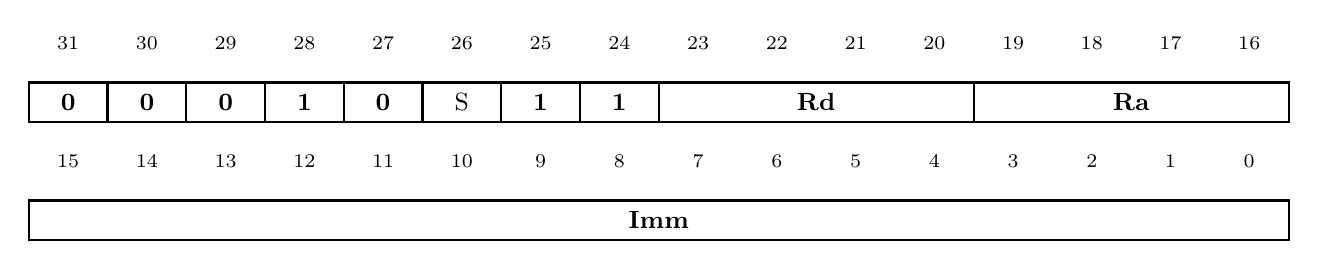
\begin{tikzpicture}
	% Bitnummern oben
	\foreach \x in {0,...,15}
		\pgfmathsetmacro{\number}{int(abs(\x-15)+16)}
		\node at (\x - 0.5, 20.5) {\scriptsize \number};
	% Bitbeschreibungen
	\filldraw[thick, draw=black, fill={rgb:white,255}] (-1, 20) rectangle (0,
	19.5);
	\node (mode) at (-0.5, 19.75) {\small \textbf{0}};
	\filldraw[thick, draw=black, fill={rgb:white,255}] (0, 20) rectangle (1,
	19.5);
	\node (mode) at (0.5, 19.75) {\small \textbf{0}};
	\filldraw[thick, draw=black, fill={rgb:white,255}] (1, 20) rectangle (2,
	19.5);
	\node (mode) at (1.5, 19.75) {\small \textbf{0}};
	\filldraw[thick, draw=black, fill={rgb:white,255}] (2, 20) rectangle (3,
	19.5);
	\node (mode) at (2.5, 19.75) {\small \textbf{1}};
	\filldraw[thick, draw=black, fill={rgb:white,255}] (3, 20) rectangle (4,
	19.5);
	\node (mode) at (3.5, 19.75) {\small \textbf{0}};
	\filldraw[thick, draw=black, fill={rgb:white,255}] (4, 20) rectangle (5,
	19.5);
	\node (mode) at (4.5, 19.75) {\small S};
	\filldraw[thick, draw=black, fill={rgb:white,255}] (5, 20) rectangle (6,
	19.5);
	\node (mode) at (5.5, 19.75) {\small \textbf{1}};
	\filldraw[thick, draw=black, fill={rgb:white,255}] (6, 20) rectangle (7,
	19.5);
	\node (mode) at (6.5, 19.75) {\small \textbf{1}};
	\filldraw[thick, draw=black, fill={rgb:white,255}] (7, 20) rectangle (11,
	19.5);
	\node (mode) at (9, 19.75) {\small \textbf{Rd}};
	\filldraw[thick, draw=black, fill={rgb:white,255}] (11, 20) rectangle (15,
	19.5);
	\node (mode) at (13, 19.75) {\small \textbf{Ra}};

	% Bitnummern oben
	\foreach \x in {0,...,15}
		\pgfmathsetmacro{\number}{int(abs(\x-15))}
		\node at (\x - 0.5, 19) {\scriptsize \number};
	% Bitbeschreibungen
	\filldraw[thick, draw=black, fill={rgb:white,255}] (-1, 18.5) rectangle (15,
	18);
	\node (mode) at (7, 18.25) {\small \textbf{Imm}};
\end{tikzpicture}

Subtrahiere eine 16-Bit-Konstante von einem Register. Das Bit \textbf{S} zeigt an,
ob die Subtraktion vorzeichenbehaftet(1) oder vorzeichenunbehaftet(0) stattfinden
soll.

\textit{Regs[Rd] = Regs[Ra] - Imm}
\section*{and}
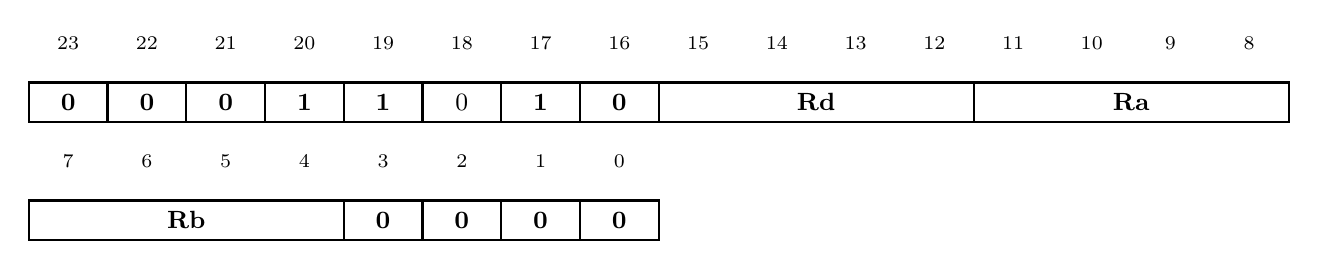
\begin{tikzpicture}
	% Bitnummern oben
	\foreach \x in {0,...,15}
		\pgfmathsetmacro{\number}{int(abs(\x-15)+8)}
		\node at (\x - 0.5, 20.5) {\scriptsize \number};
	% Bitbeschreibungen
	\filldraw[thick, draw=black, fill={rgb:white,255}] (-1, 20) rectangle (0,
	19.5);
	\node (mode) at (-0.5, 19.75) {\small \textbf{0}};
	\filldraw[thick, draw=black, fill={rgb:white,255}] (0, 20) rectangle (1,
	19.5);
	\node (mode) at (0.5, 19.75) {\small \textbf{0}};
	\filldraw[thick, draw=black, fill={rgb:white,255}] (1, 20) rectangle (2,
	19.5);
	\node (mode) at (1.5, 19.75) {\small \textbf{0}};
	\filldraw[thick, draw=black, fill={rgb:white,255}] (2, 20) rectangle (3,
	19.5);
	\node (mode) at (2.5, 19.75) {\small \textbf{1}};
	\filldraw[thick, draw=black, fill={rgb:white,255}] (3, 20) rectangle (4,
	19.5);
	\node (mode) at (3.5, 19.75) {\small \textbf{1}};
	\filldraw[thick, draw=black, fill={rgb:white,255}] (4, 20) rectangle (5,
	19.5);
	\node (mode) at (4.5, 19.75) {\small 0};
	\filldraw[thick, draw=black, fill={rgb:white,255}] (5, 20) rectangle (6,
	19.5);
	\node (mode) at (5.5, 19.75) {\small \textbf{1}};
	\filldraw[thick, draw=black, fill={rgb:white,255}] (6, 20) rectangle (7,
	19.5);
	\node (mode) at (6.5, 19.75) {\small \textbf{0}};
	\filldraw[thick, draw=black, fill={rgb:white,255}] (7, 20) rectangle (11,
	19.5);
	\node (mode) at (9, 19.75) {\small \textbf{Rd}};
	\filldraw[thick, draw=black, fill={rgb:white,255}] (11, 20) rectangle (15,
	19.5);
	\node (mode) at (13, 19.75) {\small \textbf{Ra}};

	% Bitnummern oben
	\foreach \x in {0,...,7}
		\pgfmathsetmacro{\number}{int(abs(\x-7))}
		\node at (\x - 0.5, 19) {\scriptsize \number};
	% Bitbeschreibungen
	\filldraw[thick, draw=black, fill={rgb:white,255}] (-1, 18.5) rectangle (3,
	18);
	\node (mode) at (1, 18.25) {\small \textbf{Rb}};
	\filldraw[thick, draw=black, fill={rgb:white,255}] (3, 18.5) rectangle (4,
	18);
	\node (mode) at (3.5, 18.25) {\small \textbf{0}};
	\filldraw[thick, draw=black, fill={rgb:white,255}] (4, 18.5) rectangle (5,
	18);
	\node (mode) at (4.5, 18.25) {\small \textbf{0}};
	\filldraw[thick, draw=black, fill={rgb:white,255}] (5, 18.5) rectangle (6,
	18);
	\node (mode) at (5.5, 18.25) {\small \textbf{0}};
	\filldraw[thick, draw=black, fill={rgb:white,255}] (6, 18.5) rectangle (7,
	18);
	\node (mode) at (6.5, 18.25) {\small \textbf{0}};
\end{tikzpicture}

Berechne die bitweise UND-Verknüpfung zweier Register.

\textit{Regs[Rd] = Regs[Ra] $\land$ Regs[Rb]}
\section*{or}
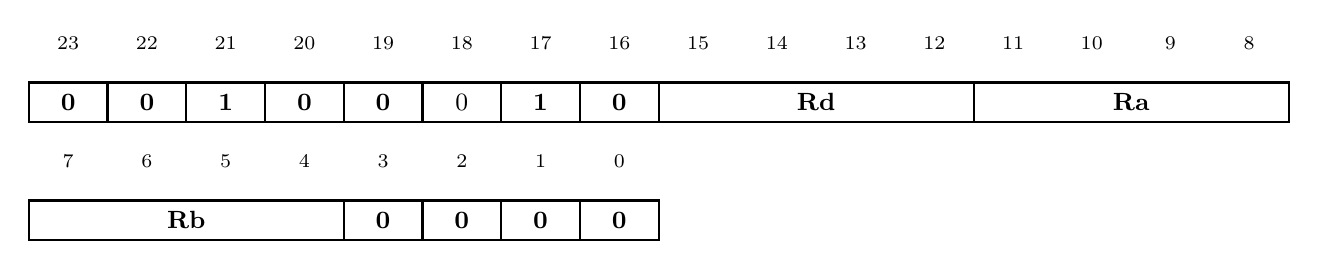
\begin{tikzpicture}
	% Bitnummern oben
	\foreach \x in {0,...,15}
		\pgfmathsetmacro{\number}{int(abs(\x-15)+8)}
		\node at (\x - 0.5, 20.5) {\scriptsize \number};
	% Bitbeschreibungen
	\filldraw[thick, draw=black, fill={rgb:white,255}] (-1, 20) rectangle (0,
	19.5);
	\node (mode) at (-0.5, 19.75) {\small \textbf{0}};
	\filldraw[thick, draw=black, fill={rgb:white,255}] (0, 20) rectangle (1,
	19.5);
	\node (mode) at (0.5, 19.75) {\small \textbf{0}};
	\filldraw[thick, draw=black, fill={rgb:white,255}] (1, 20) rectangle (2,
	19.5);
	\node (mode) at (1.5, 19.75) {\small \textbf{1}};
	\filldraw[thick, draw=black, fill={rgb:white,255}] (2, 20) rectangle (3,
	19.5);
	\node (mode) at (2.5, 19.75) {\small \textbf{0}};
	\filldraw[thick, draw=black, fill={rgb:white,255}] (3, 20) rectangle (4,
	19.5);
	\node (mode) at (3.5, 19.75) {\small \textbf{0}};
	\filldraw[thick, draw=black, fill={rgb:white,255}] (4, 20) rectangle (5,
	19.5);
	\node (mode) at (4.5, 19.75) {\small 0};
	\filldraw[thick, draw=black, fill={rgb:white,255}] (5, 20) rectangle (6,
	19.5);
	\node (mode) at (5.5, 19.75) {\small \textbf{1}};
	\filldraw[thick, draw=black, fill={rgb:white,255}] (6, 20) rectangle (7,
	19.5);
	\node (mode) at (6.5, 19.75) {\small \textbf{0}};
	\filldraw[thick, draw=black, fill={rgb:white,255}] (7, 20) rectangle (11,
	19.5);
	\node (mode) at (9, 19.75) {\small \textbf{Rd}};
	\filldraw[thick, draw=black, fill={rgb:white,255}] (11, 20) rectangle (15,
	19.5);
	\node (mode) at (13, 19.75) {\small \textbf{Ra}};

	% Bitnummern oben
	\foreach \x in {0,...,7}
		\pgfmathsetmacro{\number}{int(abs(\x-7))}
		\node at (\x - 0.5, 19) {\scriptsize \number};
	% Bitbeschreibungen
	\filldraw[thick, draw=black, fill={rgb:white,255}] (-1, 18.5) rectangle (3,
	18);
	\node (mode) at (1, 18.25) {\small \textbf{Rb}};
	\filldraw[thick, draw=black, fill={rgb:white,255}] (3, 18.5) rectangle (4,
	18);
	\node (mode) at (3.5, 18.25) {\small \textbf{0}};
	\filldraw[thick, draw=black, fill={rgb:white,255}] (4, 18.5) rectangle (5,
	18);
	\node (mode) at (4.5, 18.25) {\small \textbf{0}};
	\filldraw[thick, draw=black, fill={rgb:white,255}] (5, 18.5) rectangle (6,
	18);
	\node (mode) at (5.5, 18.25) {\small \textbf{0}};
	\filldraw[thick, draw=black, fill={rgb:white,255}] (6, 18.5) rectangle (7,
	18);
	\node (mode) at (6.5, 18.25) {\small \textbf{0}};
\end{tikzpicture}

Berechne die bitweise ODER-Verknüpfung zweier Register.

\textit{Regs[Rd] = Regs[Ra] $\lor$ Regs[Rb]}
\section*{or}
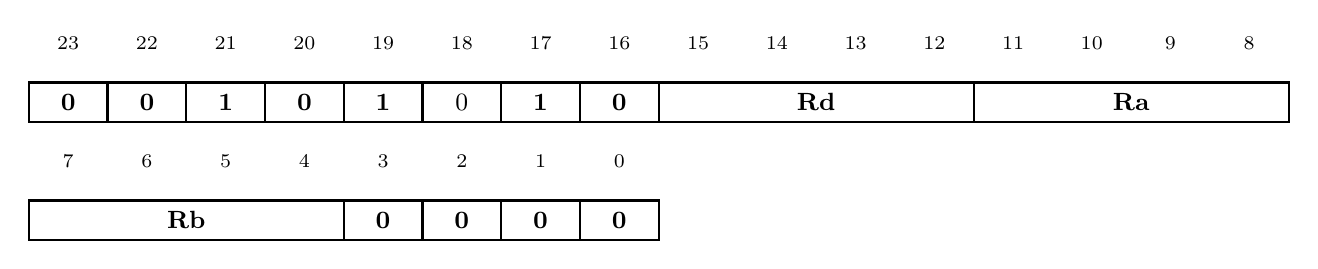
\begin{tikzpicture}
	% Bitnummern oben
	\foreach \x in {0,...,15}
		\pgfmathsetmacro{\number}{int(abs(\x-15)+8)}
		\node at (\x - 0.5, 20.5) {\scriptsize \number};
	% Bitbeschreibungen
	\filldraw[thick, draw=black, fill={rgb:white,255}] (-1, 20) rectangle (0,
	19.5);
	\node (mode) at (-0.5, 19.75) {\small \textbf{0}};
	\filldraw[thick, draw=black, fill={rgb:white,255}] (0, 20) rectangle (1,
	19.5);
	\node (mode) at (0.5, 19.75) {\small \textbf{0}};
	\filldraw[thick, draw=black, fill={rgb:white,255}] (1, 20) rectangle (2,
	19.5);
	\node (mode) at (1.5, 19.75) {\small \textbf{1}};
	\filldraw[thick, draw=black, fill={rgb:white,255}] (2, 20) rectangle (3,
	19.5);
	\node (mode) at (2.5, 19.75) {\small \textbf{0}};
	\filldraw[thick, draw=black, fill={rgb:white,255}] (3, 20) rectangle (4,
	19.5);
	\node (mode) at (3.5, 19.75) {\small \textbf{1}};
	\filldraw[thick, draw=black, fill={rgb:white,255}] (4, 20) rectangle (5,
	19.5);
	\node (mode) at (4.5, 19.75) {\small 0};
	\filldraw[thick, draw=black, fill={rgb:white,255}] (5, 20) rectangle (6,
	19.5);
	\node (mode) at (5.5, 19.75) {\small \textbf{1}};
	\filldraw[thick, draw=black, fill={rgb:white,255}] (6, 20) rectangle (7,
	19.5);
	\node (mode) at (6.5, 19.75) {\small \textbf{0}};
	\filldraw[thick, draw=black, fill={rgb:white,255}] (7, 20) rectangle (11,
	19.5);
	\node (mode) at (9, 19.75) {\small \textbf{Rd}};
	\filldraw[thick, draw=black, fill={rgb:white,255}] (11, 20) rectangle (15,
	19.5);
	\node (mode) at (13, 19.75) {\small \textbf{Ra}};

	% Bitnummern oben
	\foreach \x in {0,...,7}
		\pgfmathsetmacro{\number}{int(abs(\x-7))}
		\node at (\x - 0.5, 19) {\scriptsize \number};
	% Bitbeschreibungen
	\filldraw[thick, draw=black, fill={rgb:white,255}] (-1, 18.5) rectangle (3,
	18);
	\node (mode) at (1, 18.25) {\small \textbf{Rb}};
	\filldraw[thick, draw=black, fill={rgb:white,255}] (3, 18.5) rectangle (4,
	18);
	\node (mode) at (3.5, 18.25) {\small \textbf{0}};
	\filldraw[thick, draw=black, fill={rgb:white,255}] (4, 18.5) rectangle (5,
	18);
	\node (mode) at (4.5, 18.25) {\small \textbf{0}};
	\filldraw[thick, draw=black, fill={rgb:white,255}] (5, 18.5) rectangle (6,
	18);
	\node (mode) at (5.5, 18.25) {\small \textbf{0}};
	\filldraw[thick, draw=black, fill={rgb:white,255}] (6, 18.5) rectangle (7,
	18);
	\node (mode) at (6.5, 18.25) {\small \textbf{0}};
\end{tikzpicture}

Berechne die bitweise XOR-Verknüpfung zweier Register.

\textit{Regs[Rd] = Regs[Ra] $\oplus$ Regs[Rb]}
\section*{not}
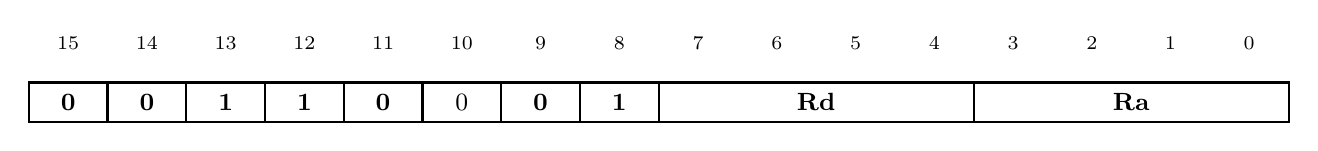
\begin{tikzpicture}
	% Bitnummern oben
	\foreach \x in {0,...,15}
		\pgfmathsetmacro{\number}{int(abs(\x-15))}
		\node at (\x - 0.5, 20.5) {\scriptsize \number};
	% Bitbeschreibungen
	\filldraw[thick, draw=black, fill={rgb:white,255}] (-1, 20) rectangle (0,
	19.5);
	\node (mode) at (-0.5, 19.75) {\small \textbf{0}};
	\filldraw[thick, draw=black, fill={rgb:white,255}] (0, 20) rectangle (1,
	19.5);
	\node (mode) at (0.5, 19.75) {\small \textbf{0}};
	\filldraw[thick, draw=black, fill={rgb:white,255}] (1, 20) rectangle (2,
	19.5);
	\node (mode) at (1.5, 19.75) {\small \textbf{1}};
	\filldraw[thick, draw=black, fill={rgb:white,255}] (2, 20) rectangle (3,
	19.5);
	\node (mode) at (2.5, 19.75) {\small \textbf{1}};
	\filldraw[thick, draw=black, fill={rgb:white,255}] (3, 20) rectangle (4,
	19.5);
	\node (mode) at (3.5, 19.75) {\small \textbf{0}};
	\filldraw[thick, draw=black, fill={rgb:white,255}] (4, 20) rectangle (5,
	19.5);
	\node (mode) at (4.5, 19.75) {\small 0};
	\filldraw[thick, draw=black, fill={rgb:white,255}] (5, 20) rectangle (6,
	19.5);
	\node (mode) at (5.5, 19.75) {\small \textbf{0}};
	\filldraw[thick, draw=black, fill={rgb:white,255}] (6, 20) rectangle (7,
	19.5);
	\node (mode) at (6.5, 19.75) {\small \textbf{1}};
	\filldraw[thick, draw=black, fill={rgb:white,255}] (7, 20) rectangle (11,
	19.5);
	\node (mode) at (9, 19.75) {\small \textbf{Rd}};
	\filldraw[thick, draw=black, fill={rgb:white,255}] (11, 20) rectangle (15,
	19.5);
	\node (mode) at (13, 19.75) {\small \textbf{Ra}};
\end{tikzpicture}

Berechne das logische NICHT eines Registers.

\textit{Regs[Rd] = $\lnot$Regs[Ra]}
\section*{load}
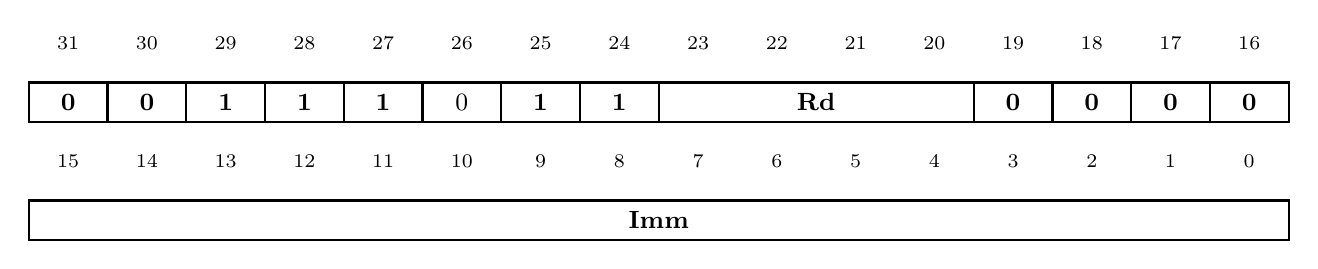
\begin{tikzpicture}
	% Bitnummern oben
	\foreach \x in {0,...,15}
		\pgfmathsetmacro{\number}{int(abs(\x-15)+16)}
		\node at (\x - 0.5, 20.5) {\scriptsize \number};
	% Bitbeschreibungen
	\filldraw[thick, draw=black, fill={rgb:white,255}] (-1, 20) rectangle (0,
	19.5);
	\node (mode) at (-0.5, 19.75) {\small \textbf{0}};
	\filldraw[thick, draw=black, fill={rgb:white,255}] (0, 20) rectangle (1,
	19.5);
	\node (mode) at (0.5, 19.75) {\small \textbf{0}};
	\filldraw[thick, draw=black, fill={rgb:white,255}] (1, 20) rectangle (2,
	19.5);
	\node (mode) at (1.5, 19.75) {\small \textbf{1}};
	\filldraw[thick, draw=black, fill={rgb:white,255}] (2, 20) rectangle (3,
	19.5);
	\node (mode) at (2.5, 19.75) {\small \textbf{1}};
	\filldraw[thick, draw=black, fill={rgb:white,255}] (3, 20) rectangle (4,
	19.5);
	\node (mode) at (3.5, 19.75) {\small \textbf{1}};
	\filldraw[thick, draw=black, fill={rgb:white,255}] (4, 20) rectangle (5,
	19.5);
	\node (mode) at (4.5, 19.75) {\small 0};
	\filldraw[thick, draw=black, fill={rgb:white,255}] (5, 20) rectangle (6,
	19.5);
	\node (mode) at (5.5, 19.75) {\small \textbf{1}};
	\filldraw[thick, draw=black, fill={rgb:white,255}] (6, 20) rectangle (7,
	19.5);
	\node (mode) at (6.5, 19.75) {\small \textbf{1}};
	\filldraw[thick, draw=black, fill={rgb:white,255}] (7, 20) rectangle (11,
	19.5);
	\node (mode) at (9, 19.75) {\small \textbf{Rd}};
	\filldraw[thick, draw=black, fill={rgb:white,255}] (11, 20) rectangle (12,
	19.5);
	\node (mode) at (11.5, 19.75) {\small \textbf{0}};
	\filldraw[thick, draw=black, fill={rgb:white,255}] (12, 20) rectangle (13,
	19.5);
	\node (mode) at (12.5, 19.75) {\small \textbf{0}};
	\filldraw[thick, draw=black, fill={rgb:white,255}] (13, 20) rectangle (14,
	19.5);
	\node (mode) at (13.5, 19.75) {\small \textbf{0}};
	\filldraw[thick, draw=black, fill={rgb:white,255}] (14, 20) rectangle (15,
	19.5);
	\node (mode) at (14.5, 19.75) {\small \textbf{0}};

	% Bitnummern oben
	\foreach \x in {0,...,15}
		\pgfmathsetmacro{\number}{int(abs(\x-15))}
		\node at (\x - 0.5, 19) {\scriptsize \number};
	% Bitbeschreibungen
	\filldraw[thick, draw=black, fill={rgb:white,255}] (-1, 18.5) rectangle (15,
	18);
	\node (mode) at (7, 18.25) {\small \textbf{Imm}};
\end{tikzpicture}

Lade eine Konstante in ein Register.

\textit{Regs[Rd] =Imm}
\section*{mov}
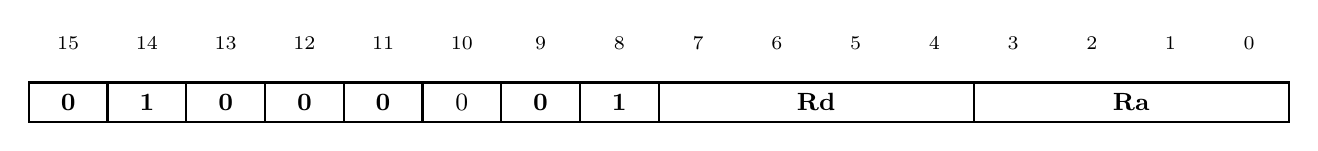
\begin{tikzpicture}
	% Bitnummern oben
	\foreach \x in {0,...,15}
		\pgfmathsetmacro{\number}{int(abs(\x-15))}
		\node at (\x - 0.5, 20.5) {\scriptsize \number};
	% Bitbeschreibungen
	\filldraw[thick, draw=black, fill={rgb:white,255}] (-1, 20) rectangle (0,
	19.5);
	\node (mode) at (-0.5, 19.75) {\small \textbf{0}};
	\filldraw[thick, draw=black, fill={rgb:white,255}] (0, 20) rectangle (1,
	19.5);
	\node (mode) at (0.5, 19.75) {\small \textbf{1}};
	\filldraw[thick, draw=black, fill={rgb:white,255}] (1, 20) rectangle (2,
	19.5);
	\node (mode) at (1.5, 19.75) {\small \textbf{0}};
	\filldraw[thick, draw=black, fill={rgb:white,255}] (2, 20) rectangle (3,
	19.5);
	\node (mode) at (2.5, 19.75) {\small \textbf{0}};
	\filldraw[thick, draw=black, fill={rgb:white,255}] (3, 20) rectangle (4,
	19.5);
	\node (mode) at (3.5, 19.75) {\small \textbf{0}};
	\filldraw[thick, draw=black, fill={rgb:white,255}] (4, 20) rectangle (5,
	19.5);
	\node (mode) at (4.5, 19.75) {\small 0};
	\filldraw[thick, draw=black, fill={rgb:white,255}] (5, 20) rectangle (6,
	19.5);
	\node (mode) at (5.5, 19.75) {\small \textbf{0}};
	\filldraw[thick, draw=black, fill={rgb:white,255}] (6, 20) rectangle (7,
	19.5);
	\node (mode) at (6.5, 19.75) {\small \textbf{1}};
	\filldraw[thick, draw=black, fill={rgb:white,255}] (7, 20) rectangle (11,
	19.5);
	\node (mode) at (9, 19.75) {\small \textbf{Rd}};
	\filldraw[thick, draw=black, fill={rgb:white,255}] (11, 20) rectangle (15,
	19.5);
	\node (mode) at (13, 19.75) {\small \textbf{Ra}};
\end{tikzpicture}

Kopiere den Wert eines Registers in ein anderes Register.

\textit{Regs[Rd] = Regs[Ra]}
\clearpage
\section*{read.l, read.h}
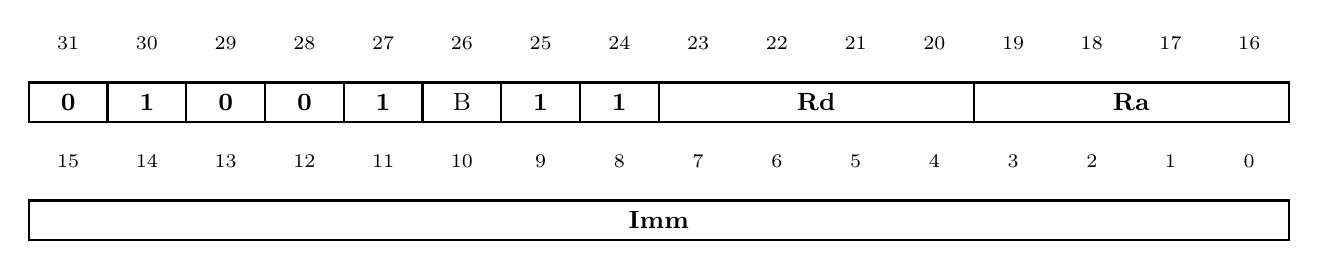
\begin{tikzpicture}
	% Bitnummern oben
	\foreach \x in {0,...,15}
		\pgfmathsetmacro{\number}{int(abs(\x-15)+16)}
		\node at (\x - 0.5, 20.5) {\scriptsize \number};
	% Bitbeschreibungen
	\filldraw[thick, draw=black, fill={rgb:white,255}] (-1, 20) rectangle (0,
	19.5);
	\node (mode) at (-0.5, 19.75) {\small \textbf{0}};
	\filldraw[thick, draw=black, fill={rgb:white,255}] (0, 20) rectangle (1,
	19.5);
	\node (mode) at (0.5, 19.75) {\small \textbf{1}};
	\filldraw[thick, draw=black, fill={rgb:white,255}] (1, 20) rectangle (2,
	19.5);
	\node (mode) at (1.5, 19.75) {\small \textbf{0}};
	\filldraw[thick, draw=black, fill={rgb:white,255}] (2, 20) rectangle (3,
	19.5);
	\node (mode) at (2.5, 19.75) {\small \textbf{0}};
	\filldraw[thick, draw=black, fill={rgb:white,255}] (3, 20) rectangle (4,
	19.5);
	\node (mode) at (3.5, 19.75) {\small \textbf{1}};
	\filldraw[thick, draw=black, fill={rgb:white,255}] (4, 20) rectangle (5,
	19.5);
	\node (mode) at (4.5, 19.75) {\small B};
	\filldraw[thick, draw=black, fill={rgb:white,255}] (5, 20) rectangle (6,
	19.5);
	\node (mode) at (5.5, 19.75) {\small \textbf{1}};
	\filldraw[thick, draw=black, fill={rgb:white,255}] (6, 20) rectangle (7,
	19.5);
	\node (mode) at (6.5, 19.75) {\small \textbf{1}};
	\filldraw[thick, draw=black, fill={rgb:white,255}] (7, 20) rectangle (11,
	19.5);
	\node (mode) at (9, 19.75) {\small \textbf{Rd}};
	\filldraw[thick, draw=black, fill={rgb:white,255}] (11, 20) rectangle (15,
	19.5);
	\node (mode) at (13, 19.75) {\small \textbf{Ra}};

	% Bitnummern oben
	\foreach \x in {0,...,15}
		\pgfmathsetmacro{\number}{int(abs(\x-15))}
		\node at (\x - 0.5, 19) {\scriptsize \number};
	% Bitbeschreibungen
	\filldraw[thick, draw=black, fill={rgb:white,255}] (-1, 18.5) rectangle (15,
	18);
	\node (mode) at (7, 18.25) {\small \textbf{Imm}};
\end{tikzpicture}

Hole den Wert vom Speicher an der angegebenen Adresse in ein Register. Die Adresse
ergibt sich aus der vorzeichenunbehafteten Addition von dem Register
\textit{Ra} und der Konstanten \textit{Imm}.

Da der Speicher immer nur ein Byte adressiert, wird mit Hilfe des Bits
\textbf{B} entschieden, ob der Wert in das untere Byte des Registers
(\textbf{B=0} bzw. \textbf{read.l}) oder in das obere Byte des Registers
(\textbf{B=1} bzw. \textbf{read.h}) geschrieben werden soll.

\textit{Regs[Rd] = Mem[Regs[Ra] + Imm]}
\section*{write.l, write.h}
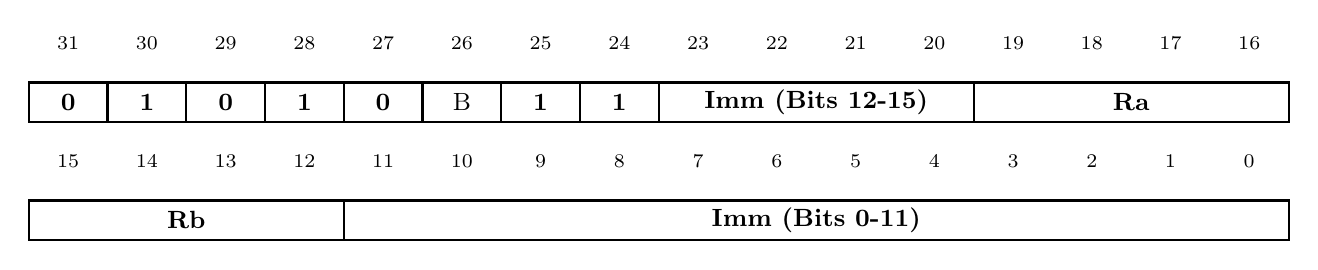
\begin{tikzpicture}
	% Bitnummern oben
	\foreach \x in {0,...,15}
		\pgfmathsetmacro{\number}{int(abs(\x-15)+16)}
		\node at (\x - 0.5, 20.5) {\scriptsize \number};
	% Bitbeschreibungen
	\filldraw[thick, draw=black, fill={rgb:white,255}] (-1, 20) rectangle (0,
	19.5);
	\node (mode) at (-0.5, 19.75) {\small \textbf{0}};
	\filldraw[thick, draw=black, fill={rgb:white,255}] (0, 20) rectangle (1,
	19.5);
	\node (mode) at (0.5, 19.75) {\small \textbf{1}};
	\filldraw[thick, draw=black, fill={rgb:white,255}] (1, 20) rectangle (2,
	19.5);
	\node (mode) at (1.5, 19.75) {\small \textbf{0}};
	\filldraw[thick, draw=black, fill={rgb:white,255}] (2, 20) rectangle (3,
	19.5);
	\node (mode) at (2.5, 19.75) {\small \textbf{1}};
	\filldraw[thick, draw=black, fill={rgb:white,255}] (3, 20) rectangle (4,
	19.5);
	\node (mode) at (3.5, 19.75) {\small \textbf{0}};
	\filldraw[thick, draw=black, fill={rgb:white,255}] (4, 20) rectangle (5,
	19.5);
	\node (mode) at (4.5, 19.75) {\small B};
	\filldraw[thick, draw=black, fill={rgb:white,255}] (5, 20) rectangle (6,
	19.5);
	\node (mode) at (5.5, 19.75) {\small \textbf{1}};
	\filldraw[thick, draw=black, fill={rgb:white,255}] (6, 20) rectangle (7,
	19.5);
	\node (mode) at (6.5, 19.75) {\small \textbf{1}};
	\filldraw[thick, draw=black, fill={rgb:white,255}] (7, 20) rectangle (11,
	19.5);
	\node (mode) at (9, 19.75) {\small \textbf{Imm (Bits 12-15)}};
	\filldraw[thick, draw=black, fill={rgb:white,255}] (11, 20) rectangle (15,
	19.5);
	\node (mode) at (13, 19.75) {\small \textbf{Ra}};

	% Bitnummern oben
	\foreach \x in {0,...,15}
		\pgfmathsetmacro{\number}{int(abs(\x-15))}
		\node at (\x - 0.5, 19) {\scriptsize \number};
	% Bitbeschreibungen
	\filldraw[thick, draw=black, fill={rgb:white,255}] (-1, 18.5) rectangle (3,
	18);
	\node (mode) at (1, 18.25) {\small \textbf{Rb}};
	\filldraw[thick, draw=black, fill={rgb:white,255}] (3, 18.5) rectangle (15,
	18);
	\node (mode) at (9, 18.25) {\small \textbf{Imm (Bits 0-11)}};
\end{tikzpicture}

Der Wert in Register \textit{Rb} wird an eine Adresse im Speicher geschrieben.
Diese Adresse ergibt sich aus der vorzeichenunbehafteten Addition von dem
Register \textit{Ra} und der Konstanten \textit{Imm}, welche aufgrund von
Optimisierungen im Dekodierer (siehe~\ref{s:decode}) getrennt vorkommt.

Da eine Speicheradresse immer nur ein Byte adressiert, wird mit dem Bit
\textbf{B} entschieden, ob das untere Byte (\textbf{B=0} bzw. \textbf{write.l})
oder das obere Byte (\textbf{B=1} bzw. \textbf{write.h}) des Registers
\textit{Rb} geschrieben wird.

\textit{Mem[Regs[Ra] + Imm] = Regs[Rb]}
\section*{shl.r}
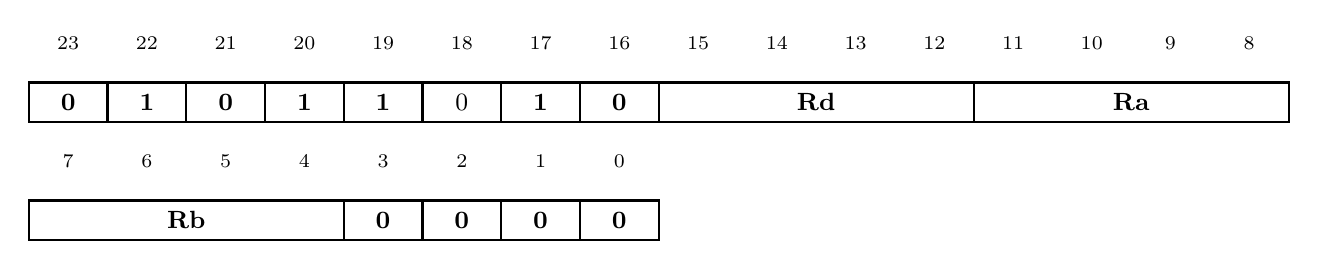
\begin{tikzpicture}
	% Bitnummern oben
	\foreach \x in {0,...,15}
		\pgfmathsetmacro{\number}{int(abs(\x-15)+8)}
		\node at (\x - 0.5, 20.5) {\scriptsize \number};
	% Bitbeschreibungen
	\filldraw[thick, draw=black, fill={rgb:white,255}] (-1, 20) rectangle (0,
	19.5);
	\node (mode) at (-0.5, 19.75) {\small \textbf{0}};
	\filldraw[thick, draw=black, fill={rgb:white,255}] (0, 20) rectangle (1,
	19.5);
	\node (mode) at (0.5, 19.75) {\small \textbf{1}};
	\filldraw[thick, draw=black, fill={rgb:white,255}] (1, 20) rectangle (2,
	19.5);
	\node (mode) at (1.5, 19.75) {\small \textbf{0}};
	\filldraw[thick, draw=black, fill={rgb:white,255}] (2, 20) rectangle (3,
	19.5);
	\node (mode) at (2.5, 19.75) {\small \textbf{1}};
	\filldraw[thick, draw=black, fill={rgb:white,255}] (3, 20) rectangle (4,
	19.5);
	\node (mode) at (3.5, 19.75) {\small \textbf{1}};
	\filldraw[thick, draw=black, fill={rgb:white,255}] (4, 20) rectangle (5,
	19.5);
	\node (mode) at (4.5, 19.75) {\small 0};
	\filldraw[thick, draw=black, fill={rgb:white,255}] (5, 20) rectangle (6,
	19.5);
	\node (mode) at (5.5, 19.75) {\small \textbf{1}};
	\filldraw[thick, draw=black, fill={rgb:white,255}] (6, 20) rectangle (7,
	19.5);
	\node (mode) at (6.5, 19.75) {\small \textbf{0}};
	\filldraw[thick, draw=black, fill={rgb:white,255}] (7, 20) rectangle (11,
	19.5);
	\node (mode) at (9, 19.75) {\small \textbf{Rd}};
	\filldraw[thick, draw=black, fill={rgb:white,255}] (11, 20) rectangle (15,
	19.5);
	\node (mode) at (13, 19.75) {\small \textbf{Ra}};

	% Bitnummern oben
	\foreach \x in {0,...,7}
		\pgfmathsetmacro{\number}{int(abs(\x-7))}
		\node at (\x - 0.5, 19) {\scriptsize \number};
	% Bitbeschreibungen
	\filldraw[thick, draw=black, fill={rgb:white,255}] (-1, 18.5) rectangle (3,
	18);
	\node (mode) at (1, 18.25) {\small \textbf{Rb}};
	\filldraw[thick, draw=black, fill={rgb:white,255}] (3, 18.5) rectangle (4,
	18);
	\node (mode) at (3.5, 18.25) {\small \textbf{0}};
	\filldraw[thick, draw=black, fill={rgb:white,255}] (4, 18.5) rectangle (5,
	18);
	\node (mode) at (4.5, 18.25) {\small \textbf{0}};
	\filldraw[thick, draw=black, fill={rgb:white,255}] (5, 18.5) rectangle (6,
	18);
	\node (mode) at (5.5, 18.25) {\small \textbf{0}};
	\filldraw[thick, draw=black, fill={rgb:white,255}] (6, 18.5) rectangle (7,
	18);
	\node (mode) at (6.5, 18.25) {\small \textbf{0}};
\end{tikzpicture}

Dieser Befehl führt eine logische Verschiebung nach links um einen bestimmten
Wert aus. Dieser Wert wird aus dem Register \textit{Rb} genommen.

\textit{Regs[Rd] = Regs[Ra] << Regs[Rb]}
\section*{shl.i}
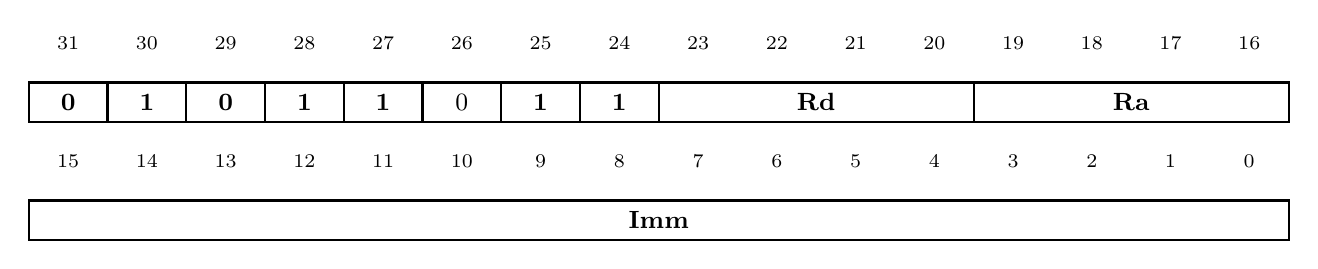
\begin{tikzpicture}
	% Bitnummern oben
	\foreach \x in {0,...,15}
		\pgfmathsetmacro{\number}{int(abs(\x-15)+16)}
		\node at (\x - 0.5, 20.5) {\scriptsize \number};
	% Bitbeschreibungen
	\filldraw[thick, draw=black, fill={rgb:white,255}] (-1, 20) rectangle (0,
	19.5);
	\node (mode) at (-0.5, 19.75) {\small \textbf{0}};
	\filldraw[thick, draw=black, fill={rgb:white,255}] (0, 20) rectangle (1,
	19.5);
	\node (mode) at (0.5, 19.75) {\small \textbf{1}};
	\filldraw[thick, draw=black, fill={rgb:white,255}] (1, 20) rectangle (2,
	19.5);
	\node (mode) at (1.5, 19.75) {\small \textbf{0}};
	\filldraw[thick, draw=black, fill={rgb:white,255}] (2, 20) rectangle (3,
	19.5);
	\node (mode) at (2.5, 19.75) {\small \textbf{1}};
	\filldraw[thick, draw=black, fill={rgb:white,255}] (3, 20) rectangle (4,
	19.5);
	\node (mode) at (3.5, 19.75) {\small \textbf{1}};
	\filldraw[thick, draw=black, fill={rgb:white,255}] (4, 20) rectangle (5,
	19.5);
	\node (mode) at (4.5, 19.75) {\small 0};
	\filldraw[thick, draw=black, fill={rgb:white,255}] (5, 20) rectangle (6,
	19.5);
	\node (mode) at (5.5, 19.75) {\small \textbf{1}};
	\filldraw[thick, draw=black, fill={rgb:white,255}] (6, 20) rectangle (7,
	19.5);
	\node (mode) at (6.5, 19.75) {\small \textbf{1}};
	\filldraw[thick, draw=black, fill={rgb:white,255}] (7, 20) rectangle (11,
	19.5);
	\node (mode) at (9, 19.75) {\small \textbf{Rd}};
	\filldraw[thick, draw=black, fill={rgb:white,255}] (11, 20) rectangle (15,
	19.5);
	\node (mode) at (13, 19.75) {\small \textbf{Ra}};

	% Bitnummern oben
	\foreach \x in {0,...,15}
		\pgfmathsetmacro{\number}{int(abs(\x-15))}
		\node at (\x - 0.5, 19) {\scriptsize \number};
	% Bitbeschreibungen
	\filldraw[thick, draw=black, fill={rgb:white,255}] (-1, 18.5) rectangle (15,
	18);
	\node (mode) at (7, 18.25) {\small \textbf{Imm}};
\end{tikzpicture}

Dieser Befehl führt eine logische Verschiebung nach links um einen bestimmten
Wert aus. Dieser Wert wird von der Konstante \textit{Imm} genommen.

\textit{Regs[Rd] = Regs[Ra] << Imm]}
\section*{shr.r}
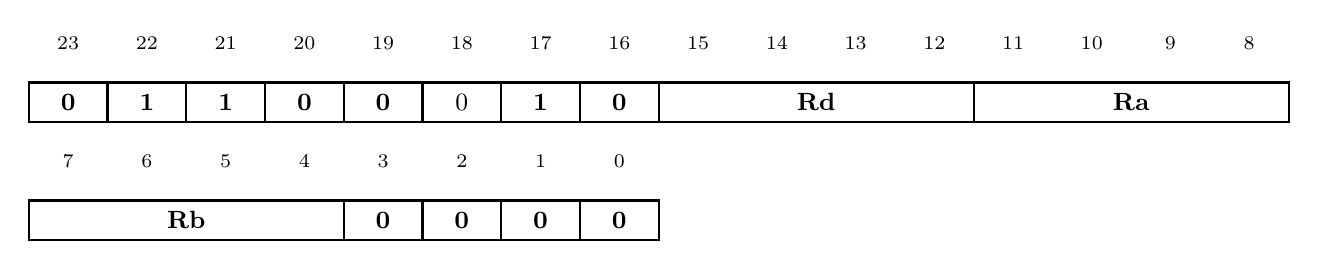
\begin{tikzpicture}
	% Bitnummern oben
	\foreach \x in {0,...,15}
		\pgfmathsetmacro{\number}{int(abs(\x-15)+8)}
		\node at (\x - 0.5, 20.5) {\scriptsize \number};
	% Bitbeschreibungen
	\filldraw[thick, draw=black, fill={rgb:white,255}] (-1, 20) rectangle (0,
	19.5);
	\node (mode) at (-0.5, 19.75) {\small \textbf{0}};
	\filldraw[thick, draw=black, fill={rgb:white,255}] (0, 20) rectangle (1,
	19.5);
	\node (mode) at (0.5, 19.75) {\small \textbf{1}};
	\filldraw[thick, draw=black, fill={rgb:white,255}] (1, 20) rectangle (2,
	19.5);
	\node (mode) at (1.5, 19.75) {\small \textbf{1}};
	\filldraw[thick, draw=black, fill={rgb:white,255}] (2, 20) rectangle (3,
	19.5);
	\node (mode) at (2.5, 19.75) {\small \textbf{0}};
	\filldraw[thick, draw=black, fill={rgb:white,255}] (3, 20) rectangle (4,
	19.5);
	\node (mode) at (3.5, 19.75) {\small \textbf{0}};
	\filldraw[thick, draw=black, fill={rgb:white,255}] (4, 20) rectangle (5,
	19.5);
	\node (mode) at (4.5, 19.75) {\small 0};
	\filldraw[thick, draw=black, fill={rgb:white,255}] (5, 20) rectangle (6,
	19.5);
	\node (mode) at (5.5, 19.75) {\small \textbf{1}};
	\filldraw[thick, draw=black, fill={rgb:white,255}] (6, 20) rectangle (7,
	19.5);
	\node (mode) at (6.5, 19.75) {\small \textbf{0}};
	\filldraw[thick, draw=black, fill={rgb:white,255}] (7, 20) rectangle (11,
	19.5);
	\node (mode) at (9, 19.75) {\small \textbf{Rd}};
	\filldraw[thick, draw=black, fill={rgb:white,255}] (11, 20) rectangle (15,
	19.5);
	\node (mode) at (13, 19.75) {\small \textbf{Ra}};

	% Bitnummern oben
	\foreach \x in {0,...,7}
		\pgfmathsetmacro{\number}{int(abs(\x-7))}
		\node at (\x - 0.5, 19) {\scriptsize \number};
	% Bitbeschreibungen
	\filldraw[thick, draw=black, fill={rgb:white,255}] (-1, 18.5) rectangle (3,
	18);
	\node (mode) at (1, 18.25) {\small \textbf{Rb}};
	\filldraw[thick, draw=black, fill={rgb:white,255}] (3, 18.5) rectangle (4,
	18);
	\node (mode) at (3.5, 18.25) {\small \textbf{0}};
	\filldraw[thick, draw=black, fill={rgb:white,255}] (4, 18.5) rectangle (5,
	18);
	\node (mode) at (4.5, 18.25) {\small \textbf{0}};
	\filldraw[thick, draw=black, fill={rgb:white,255}] (5, 18.5) rectangle (6,
	18);
	\node (mode) at (5.5, 18.25) {\small \textbf{0}};
	\filldraw[thick, draw=black, fill={rgb:white,255}] (6, 18.5) rectangle (7,
	18);
	\node (mode) at (6.5, 18.25) {\small \textbf{0}};
\end{tikzpicture}

Dieser Befehl führt eine logische Verschiebung nach rechts um einen bestimmten
Wert aus. Dieser Wert wird aus dem Register \textit{Rb} genommen.

\textit{Regs[Rd] = Regs[Ra] >> Regs[Rb]}
\section*{shr.i}
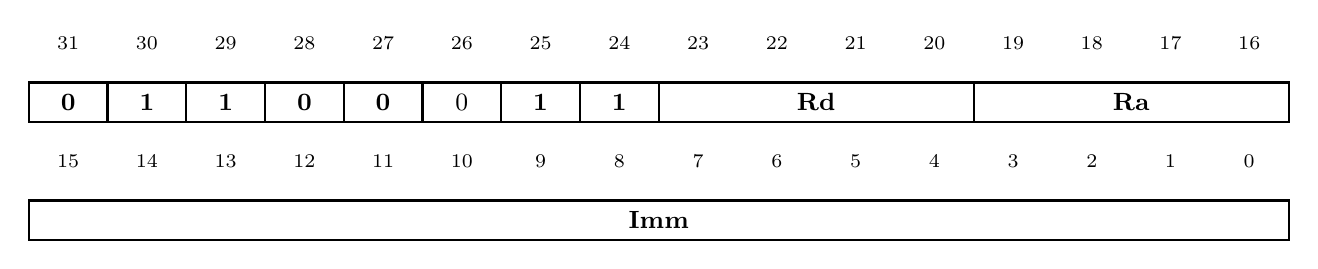
\begin{tikzpicture}
	% Bitnummern oben
	\foreach \x in {0,...,15}
		\pgfmathsetmacro{\number}{int(abs(\x-15)+16)}
		\node at (\x - 0.5, 20.5) {\scriptsize \number};
	% Bitbeschreibungen
	\filldraw[thick, draw=black, fill={rgb:white,255}] (-1, 20) rectangle (0,
	19.5);
	\node (mode) at (-0.5, 19.75) {\small \textbf{0}};
	\filldraw[thick, draw=black, fill={rgb:white,255}] (0, 20) rectangle (1,
	19.5);
	\node (mode) at (0.5, 19.75) {\small \textbf{1}};
	\filldraw[thick, draw=black, fill={rgb:white,255}] (1, 20) rectangle (2,
	19.5);
	\node (mode) at (1.5, 19.75) {\small \textbf{1}};
	\filldraw[thick, draw=black, fill={rgb:white,255}] (2, 20) rectangle (3,
	19.5);
	\node (mode) at (2.5, 19.75) {\small \textbf{0}};
	\filldraw[thick, draw=black, fill={rgb:white,255}] (3, 20) rectangle (4,
	19.5);
	\node (mode) at (3.5, 19.75) {\small \textbf{0}};
	\filldraw[thick, draw=black, fill={rgb:white,255}] (4, 20) rectangle (5,
	19.5);
	\node (mode) at (4.5, 19.75) {\small 0};
	\filldraw[thick, draw=black, fill={rgb:white,255}] (5, 20) rectangle (6,
	19.5);
	\node (mode) at (5.5, 19.75) {\small \textbf{1}};
	\filldraw[thick, draw=black, fill={rgb:white,255}] (6, 20) rectangle (7,
	19.5);
	\node (mode) at (6.5, 19.75) {\small \textbf{1}};
	\filldraw[thick, draw=black, fill={rgb:white,255}] (7, 20) rectangle (11,
	19.5);
	\node (mode) at (9, 19.75) {\small \textbf{Rd}};
	\filldraw[thick, draw=black, fill={rgb:white,255}] (11, 20) rectangle (15,
	19.5);
	\node (mode) at (13, 19.75) {\small \textbf{Ra}};

	% Bitnummern oben
	\foreach \x in {0,...,15}
		\pgfmathsetmacro{\number}{int(abs(\x-15))}
		\node at (\x - 0.5, 19) {\scriptsize \number};
	% Bitbeschreibungen
	\filldraw[thick, draw=black, fill={rgb:white,255}] (-1, 18.5) rectangle (15,
	18);
	\node (mode) at (7, 18.25) {\small \textbf{Imm}};
\end{tikzpicture}

Dieser Befehl führt eine logische Verschiebung nach rechts um einen bestimmten
Wert aus. Dieser Wert wird von der Konstante \textit{Imm} genommen.

\textit{Regs[Rd] = Regs[Ra] >> Imm}
\section*{cmp.u, cmp.s}
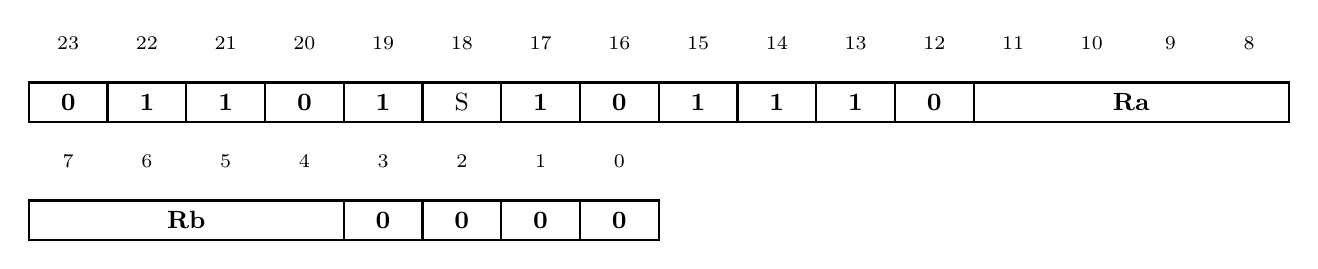
\begin{tikzpicture}
	% Bitnummern oben
	\foreach \x in {0,...,15}
		\pgfmathsetmacro{\number}{int(abs(\x-15)+8)}
		\node at (\x - 0.5, 20.5) {\scriptsize \number};
	% Bitbeschreibungen
	\filldraw[thick, draw=black, fill={rgb:white,255}] (-1, 20) rectangle (0,
	19.5);
	\node (mode) at (-0.5, 19.75) {\small \textbf{0}};
	\filldraw[thick, draw=black, fill={rgb:white,255}] (0, 20) rectangle (1,
	19.5);
	\node (mode) at (0.5, 19.75) {\small \textbf{1}};
	\filldraw[thick, draw=black, fill={rgb:white,255}] (1, 20) rectangle (2,
	19.5);
	\node (mode) at (1.5, 19.75) {\small \textbf{1}};
	\filldraw[thick, draw=black, fill={rgb:white,255}] (2, 20) rectangle (3,
	19.5);
	\node (mode) at (2.5, 19.75) {\small \textbf{0}};
	\filldraw[thick, draw=black, fill={rgb:white,255}] (3, 20) rectangle (4,
	19.5);
	\node (mode) at (3.5, 19.75) {\small \textbf{1}};
	\filldraw[thick, draw=black, fill={rgb:white,255}] (4, 20) rectangle (5,
	19.5);
	\node (mode) at (4.5, 19.75) {\small S};
	\filldraw[thick, draw=black, fill={rgb:white,255}] (5, 20) rectangle (6,
	19.5);
	\node (mode) at (5.5, 19.75) {\small \textbf{1}};
	\filldraw[thick, draw=black, fill={rgb:white,255}] (6, 20) rectangle (7,
	19.5);
	\node (mode) at (6.5, 19.75) {\small \textbf{0}};
	\filldraw[thick, draw=black, fill={rgb:white,255}] (7, 20) rectangle (8,
	19.5);
	\node (mode) at (7.5, 19.75) {\small \textbf{1}};
	\filldraw[thick, draw=black, fill={rgb:white,255}] (8, 20) rectangle (9,
	19.5);
	\node (mode) at (8.5, 19.75) {\small \textbf{1}};
	\filldraw[thick, draw=black, fill={rgb:white,255}] (9, 20) rectangle (10,
	19.5);
	\node (mode) at (9.5, 19.75) {\small \textbf{1}};
	\filldraw[thick, draw=black, fill={rgb:white,255}] (10, 20) rectangle (11,
	19.5);
	\node (mode) at (10.5, 19.75) {\small \textbf{0}};
	\filldraw[thick, draw=black, fill={rgb:white,255}] (11, 20) rectangle (15,
	19.5);
	\node (mode) at (13, 19.75) {\small \textbf{Ra}};

	% Bitnummern oben
	\foreach \x in {0,...,7}
		\pgfmathsetmacro{\number}{int(abs(\x-7))}
		\node at (\x - 0.5, 19) {\scriptsize \number};
	% Bitbeschreibungen
	\filldraw[thick, draw=black, fill={rgb:white,255}] (-1, 18.5) rectangle (3,
	18);
	\node (mode) at (1, 18.25) {\small \textbf{Rb}};
	\filldraw[thick, draw=black, fill={rgb:white,255}] (3, 18.5) rectangle (4,
	18);
	\node (mode) at (3.5, 18.25) {\small \textbf{0}};
	\filldraw[thick, draw=black, fill={rgb:white,255}] (4, 18.5) rectangle (5,
	18);
	\node (mode) at (4.5, 18.25) {\small \textbf{0}};
	\filldraw[thick, draw=black, fill={rgb:white,255}] (5, 18.5) rectangle (6,
	18);
	\node (mode) at (5.5, 18.25) {\small \textbf{0}};
	\filldraw[thick, draw=black, fill={rgb:white,255}] (6, 18.5) rectangle (7,
	18);
	\node (mode) at (6.5, 18.25) {\small \textbf{0}};
\end{tikzpicture}

Vergleiche zwei Register und speichere die Vergleichsbitmaske in Register
\textbf{R14}.

\textit{Regs[14] = cmp(Regs[Ra], Regs[Rb])}

\subsubsection*{Vergleichsbitmaske}
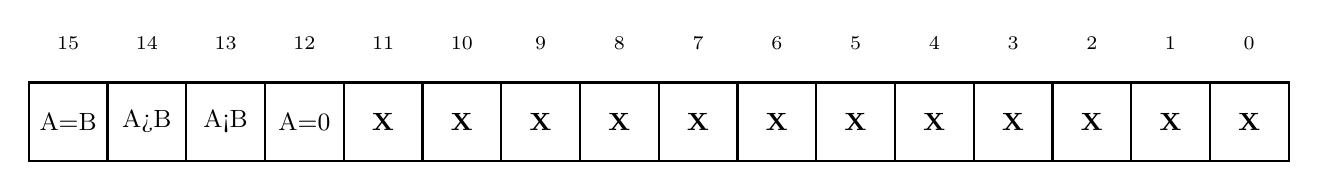
\begin{tikzpicture}
	% Bitnummern oben
	\foreach \x in {0,...,15}
		\pgfmathsetmacro{\number}{int(abs(\x-15))}
		\node at (\x - 0.5, 20.5) {\scriptsize \number};
	% Bitbeschreibungen
	\filldraw[thick, draw=black, fill={rgb:white,255}] (-1, 20) rectangle (0,
	19);
	\node (mode) at (-0.5, 19.5) {\small A=B};
	\filldraw[thick, draw=black, fill={rgb:white,255}] (0, 20) rectangle (1,
	19);
	\node (mode) at (0.5, 19.5) {\small A>B};
	\filldraw[thick, draw=black, fill={rgb:white,255}] (1, 20) rectangle (2,
	19);
	\node (mode) at (1.5, 19.5) {\small A<B};
	\filldraw[thick, draw=black, fill={rgb:white,255}] (2, 20) rectangle (3,
	19);
	\node (mode) at (2.5, 19.5) {\small A=0};
	\filldraw[thick, draw=black, fill={rgb:white,255}] (3, 20) rectangle (4,
	19);
	\node (mode) at (3.5, 19.5) {\small \textbf{X}};
	\filldraw[thick, draw=black, fill={rgb:white,255}] (4, 20) rectangle (5,
	19);
	\node (mode) at (4.5, 19.5) {\small \textbf{X}};
	\filldraw[thick, draw=black, fill={rgb:white,255}] (5, 20) rectangle (6,
	19);
	\node (mode) at (5.5, 19.5) {\small \textbf{X}};
	\filldraw[thick, draw=black, fill={rgb:white,255}] (6, 20) rectangle (7,
	19);
	\node (mode) at (6.5, 19.5) {\small \textbf{X}};
	\filldraw[thick, draw=black, fill={rgb:white,255}] (7, 20) rectangle (8,
	19);
	\node (mode) at (7.5, 19.5) {\small \textbf{X}};
	\filldraw[thick, draw=black, fill={rgb:white,255}] (8, 20) rectangle (9,
	19);
	\node (mode) at (8.5, 19.5) {\small \textbf{X}};
	\filldraw[thick, draw=black, fill={rgb:white,255}] (9, 20) rectangle (10,
	19);
	\node (mode) at (9.5, 19.5) {\small \textbf{X}};
	\filldraw[thick, draw=black, fill={rgb:white,255}] (10, 20) rectangle (11,
	19);
	\node (mode) at (10.5, 19.5) {\small \textbf{X}};
	\filldraw[thick, draw=black, fill={rgb:white,255}] (11, 20) rectangle (12,
	19);
	\node (mode) at (11.5, 19.5) {\small \textbf{X}};
	\filldraw[thick, draw=black, fill={rgb:white,255}] (12, 20) rectangle (13,
	19);
	\node (mode) at (12.5, 19.5) {\small \textbf{X}};
	\filldraw[thick, draw=black, fill={rgb:white,255}] (13, 20) rectangle (14,
	19);
	\node (mode) at (13.5, 19.5) {\small \textbf{X}};
	\filldraw[thick, draw=black, fill={rgb:white,255}] (14, 20) rectangle (15,
	19);
	\node (mode) at (14.5, 19.5) {\small \textbf{X}};
\end{tikzpicture}
\section*{jmp.r}
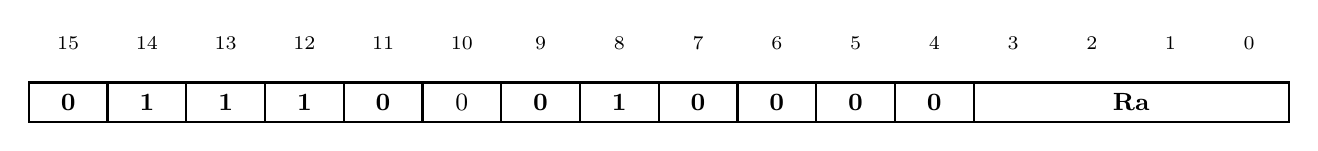
\begin{tikzpicture}
	% Bitnummern oben
	\foreach \x in {0,...,15}
		\pgfmathsetmacro{\number}{int(abs(\x-15))}
		\node at (\x - 0.5, 20.5) {\scriptsize \number};
	% Bitbeschreibungen
	\filldraw[thick, draw=black, fill={rgb:white,255}] (-1, 20) rectangle (0,
	19.5);
	\node (mode) at (-0.5, 19.75) {\small \textbf{0}};
	\filldraw[thick, draw=black, fill={rgb:white,255}] (0, 20) rectangle (1,
	19.5);
	\node (mode) at (0.5, 19.75) {\small \textbf{1}};
	\filldraw[thick, draw=black, fill={rgb:white,255}] (1, 20) rectangle (2,
	19.5);
	\node (mode) at (1.5, 19.75) {\small \textbf{1}};
	\filldraw[thick, draw=black, fill={rgb:white,255}] (2, 20) rectangle (3,
	19.5);
	\node (mode) at (2.5, 19.75) {\small \textbf{1}};
	\filldraw[thick, draw=black, fill={rgb:white,255}] (3, 20) rectangle (4,
	19.5);
	\node (mode) at (3.5, 19.75) {\small \textbf{0}};
	\filldraw[thick, draw=black, fill={rgb:white,255}] (4, 20) rectangle (5,
	19.5);
	\node (mode) at (4.5, 19.75) {\small 0};
	\filldraw[thick, draw=black, fill={rgb:white,255}] (5, 20) rectangle (6,
	19.5);
	\node (mode) at (5.5, 19.75) {\small \textbf{0}};
	\filldraw[thick, draw=black, fill={rgb:white,255}] (6, 20) rectangle (7,
	19.5);
	\node (mode) at (6.5, 19.75) {\small \textbf{1}};
	\filldraw[thick, draw=black, fill={rgb:white,255}] (7, 20) rectangle (8,
	19.5);
	\node (mode) at (7.5, 19.75) {\small \textbf{0}};
	\filldraw[thick, draw=black, fill={rgb:white,255}] (8, 20) rectangle (9,
	19.5);
	\node (mode) at (8.5, 19.75) {\small \textbf{0}};
	\filldraw[thick, draw=black, fill={rgb:white,255}] (9, 20) rectangle (10,
	19.5);
	\node (mode) at (9.5, 19.75) {\small \textbf{0}};
	\filldraw[thick, draw=black, fill={rgb:white,255}] (10, 20) rectangle (11,
	19.5);
	\node (mode) at (10.5, 19.75) {\small \textbf{0}};
	\filldraw[thick, draw=black, fill={rgb:white,255}] (11, 20) rectangle (15,
	19.5);
	\node (mode) at (13, 19.75) {\small \textbf{Ra}};
\end{tikzpicture}

Springe zu Adresse. Die Adresse wird durch das Register \textit{Ra} gegeben.

\textit{PC = Regs[Ra]}
\section*{jmp.o, jmp.i}
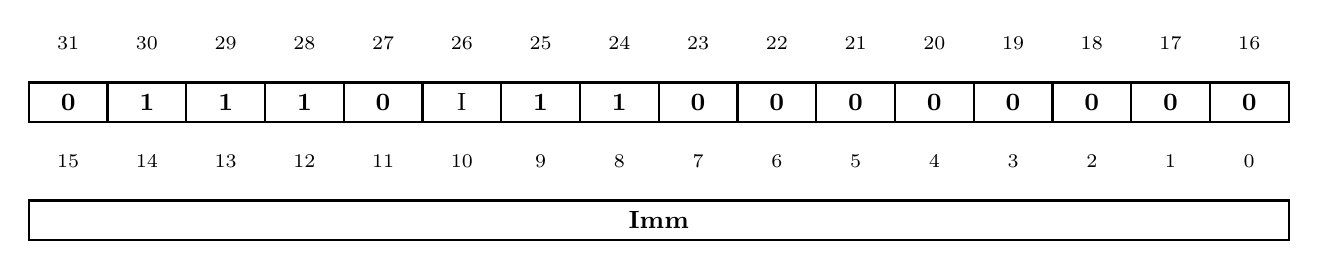
\begin{tikzpicture}
	% Bitnummern oben
	\foreach \x in {0,...,15}
		\pgfmathsetmacro{\number}{int(abs(\x-15)+16)}
		\node at (\x - 0.5, 20.5) {\scriptsize \number};
	% Bitbeschreibungen
	\filldraw[thick, draw=black, fill={rgb:white,255}] (-1, 20) rectangle (0,
	19.5);
	\node (mode) at (-0.5, 19.75) {\small \textbf{0}};
	\filldraw[thick, draw=black, fill={rgb:white,255}] (0, 20) rectangle (1,
	19.5);
	\node (mode) at (0.5, 19.75) {\small \textbf{1}};
	\filldraw[thick, draw=black, fill={rgb:white,255}] (1, 20) rectangle (2,
	19.5);
	\node (mode) at (1.5, 19.75) {\small \textbf{1}};
	\filldraw[thick, draw=black, fill={rgb:white,255}] (2, 20) rectangle (3,
	19.5);
	\node (mode) at (2.5, 19.75) {\small \textbf{1}};
	\filldraw[thick, draw=black, fill={rgb:white,255}] (3, 20) rectangle (4,
	19.5);
	\node (mode) at (3.5, 19.75) {\small \textbf{0}};
	\filldraw[thick, draw=black, fill={rgb:white,255}] (4, 20) rectangle (5,
	19.5);
	\node (mode) at (4.5, 19.75) {\small I};
	\filldraw[thick, draw=black, fill={rgb:white,255}] (5, 20) rectangle (6,
	19.5);
	\node (mode) at (5.5, 19.75) {\small \textbf{1}};
	\filldraw[thick, draw=black, fill={rgb:white,255}] (6, 20) rectangle (7,
	19.5);
	\node (mode) at (6.5, 19.75) {\small \textbf{1}};
	\filldraw[thick, draw=black, fill={rgb:white,255}] (7, 20) rectangle (8,
	19.5);
	\node (mode) at (7.5, 19.75) {\small \textbf{0}};
	\filldraw[thick, draw=black, fill={rgb:white,255}] (8, 20) rectangle (9,
	19.5);
	\node (mode) at (8.5, 19.75) {\small \textbf{0}};
	\filldraw[thick, draw=black, fill={rgb:white,255}] (9, 20) rectangle (10,
	19.5);
	\node (mode) at (9.5, 19.75) {\small \textbf{0}};
	\filldraw[thick, draw=black, fill={rgb:white,255}] (10, 20) rectangle (11,
	19.5);
	\node (mode) at (10.5, 19.75) {\small \textbf{0}};
	\filldraw[thick, draw=black, fill={rgb:white,255}] (11, 20) rectangle (12,
	19.5);
	\node (mode) at (11.5, 19.75) {\small \textbf{0}};
	\filldraw[thick, draw=black, fill={rgb:white,255}] (12, 20) rectangle (13,
	19.5);
	\node (mode) at (12.5, 19.75) {\small \textbf{0}};
	\filldraw[thick, draw=black, fill={rgb:white,255}] (13, 20) rectangle (14,
	19.5);
	\node (mode) at (13.5, 19.75) {\small \textbf{0}};
	\filldraw[thick, draw=black, fill={rgb:white,255}] (14, 20) rectangle (15,
	19.5);
	\node (mode) at (14.5, 19.75) {\small \textbf{0}};

	% Bitnummern oben
	\foreach \x in {0,...,15}
		\pgfmathsetmacro{\number}{int(abs(\x-15))}
		\node at (\x - 0.5, 19) {\scriptsize \number};
	% Bitbeschreibungen
	\filldraw[thick, draw=black, fill={rgb:white,255}] (-1, 18.5) rectangle (15,
	18);
	\node (mode) at (7, 18.25) {\small \textbf{Imm}};
\end{tikzpicture}

Springe zu Adresse. Wenn das Bit \textbf{I} gesetzt ist, wird der Wert der
Konstante \textit{Imm} als Adresse übernommen (1), andernfalls wird der Wert zum
derzeitigen Wert des PC's addiert (2). Dabei wird im zweiten Fall immer von
vorzeichenbehafteten Zahlen ausgegangen, damit auch Sprünge rückwarts
stattfinden können.

(1) \textit{PC = Imm}

(2) \textit{PC = PC + Imm}
\section*{je.r, jne.r, jg.r, jl.r jge.r, jle.r, jp.r, jnp.r, jc.r, jnc.r, jo.r,
	jno.r, jz.r, jnz.r, jb.r, jnb.r}
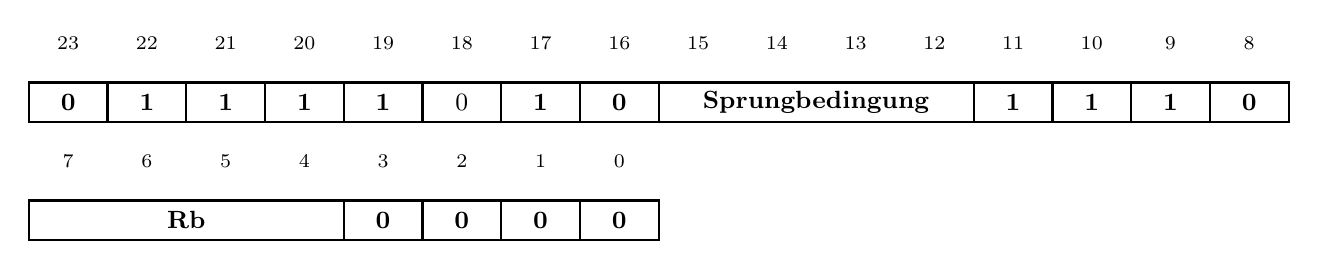
\begin{tikzpicture}
	% Bitnummern oben
	\foreach \x in {0,...,15}
		\pgfmathsetmacro{\number}{int(abs(\x-15)+8)}
		\node at (\x - 0.5, 20.5) {\scriptsize \number};
	% Bitbeschreibungen
	\filldraw[thick, draw=black, fill={rgb:white,255}] (-1, 20) rectangle (0,
	19.5);
	\node (mode) at (-0.5, 19.75) {\small \textbf{0}};
	\filldraw[thick, draw=black, fill={rgb:white,255}] (0, 20) rectangle (1,
	19.5);
	\node (mode) at (0.5, 19.75) {\small \textbf{1}};
	\filldraw[thick, draw=black, fill={rgb:white,255}] (1, 20) rectangle (2,
	19.5);
	\node (mode) at (1.5, 19.75) {\small \textbf{1}};
	\filldraw[thick, draw=black, fill={rgb:white,255}] (2, 20) rectangle (3,
	19.5);
	\node (mode) at (2.5, 19.75) {\small \textbf{1}};
	\filldraw[thick, draw=black, fill={rgb:white,255}] (3, 20) rectangle (4,
	19.5);
	\node (mode) at (3.5, 19.75) {\small \textbf{1}};
	\filldraw[thick, draw=black, fill={rgb:white,255}] (4, 20) rectangle (5,
	19.5);
	\node (mode) at (4.5, 19.75) {\small 0};
	\filldraw[thick, draw=black, fill={rgb:white,255}] (5, 20) rectangle (6,
	19.5);
	\node (mode) at (5.5, 19.75) {\small \textbf{1}};
	\filldraw[thick, draw=black, fill={rgb:white,255}] (6, 20) rectangle (7,
	19.5);
	\node (mode) at (6.5, 19.75) {\small \textbf{0}};
	\filldraw[thick, draw=black, fill={rgb:white,255}] (7, 20) rectangle (11,
	19.5);
	\node (mode) at (9, 19.75) {\small \textbf{Sprungbedingung}};
	\filldraw[thick, draw=black, fill={rgb:white,255}] (11, 20) rectangle (12,
	19.5);
	\node (mode) at (11.5, 19.75) {\small \textbf{1}};
	\filldraw[thick, draw=black, fill={rgb:white,255}] (12, 20) rectangle (13,
	19.5);
	\node (mode) at (12.5, 19.75) {\small \textbf{1}};
	\filldraw[thick, draw=black, fill={rgb:white,255}] (13, 20) rectangle (14,
	19.5);
	\node (mode) at (13.5, 19.75) {\small \textbf{1}};
	\filldraw[thick, draw=black, fill={rgb:white,255}] (14, 20) rectangle (15,
	19.5);
	\node (mode) at (14.5, 19.75) {\small \textbf{0}};

	% Bitnummern oben
	\foreach \x in {0,...,7}
		\pgfmathsetmacro{\number}{int(abs(\x-7))}
		\node at (\x - 0.5, 19) {\scriptsize \number};
	% Bitbeschreibungen
	\filldraw[thick, draw=black, fill={rgb:white,255}] (-1, 18.5) rectangle (3,
	18);
	\node (mode) at (1, 18.25) {\small \textbf{Rb}};
	\filldraw[thick, draw=black, fill={rgb:white,255}] (3, 18.5) rectangle (4,
	18);
	\node (mode) at (3.5, 18.25) {\small \textbf{0}};
	\filldraw[thick, draw=black, fill={rgb:white,255}] (4, 18.5) rectangle (5,
	18);
	\node (mode) at (4.5, 18.25) {\small \textbf{0}};
	\filldraw[thick, draw=black, fill={rgb:white,255}] (5, 18.5) rectangle (6,
	18);
	\node (mode) at (5.5, 18.25) {\small \textbf{0}};
	\filldraw[thick, draw=black, fill={rgb:white,255}] (6, 18.5) rectangle (7,
	18);
	\node (mode) at (6.5, 18.25) {\small \textbf{0}};
\end{tikzpicture}

Springe zu Adresse, wenn die \textit{Sprungbedingung} erfüllt ist. Die Adresse
wird aus dem Register \textit{Rb} gelesen. Zur Überprüfung der Sprungbedingung
wird diese mit dem Register \textbf{R14} verglichen, welches das Ergebnis der
\textbf{Vergleichsbitmaske} bzw. \textbf{Testbitmaske} enthält (siehe Befehl
\textit{cmp}). Mehr Informationen zur Sprungbedingung können der
Tabelle~\ref{tab:sprungbedingung} entnommen werden.

\textit{Regs[14] = cmp(Regs[Ra], Regs[Rb])}

\begin{table}[!htb]
\centering
\begin{tabular}{lll}
\toprule
Bitmuster & Befehl & Bedingung\\
\midrule
0000 & je  & A == B\\
0001 & jne  & A != B\\
0010 & jg  & A > B\\
0011 & jl  & A < B\\
0100 & jge  & A >= B\\
0101 & jle  & A <= B\\
0110 & jp  & Paritätsbit von A ist gesetzt\\
0111 & jnp  & Paritätsbit von A ist nicht gesetzt\\
1000 & jc  & Carrybit gesetzt\\
1001 & jnc  & Carrybit nicht gesetzt\\
1010 & jo & Überlaufbit gesetzt\\
1011 & jno & Überlaufbit nicht gesetzt\\
1100 & jz & A == 0\\
1101 & jnz & A != 0\\
1110 & jb & Bit gesetzt\\
1111 & jnb  & Bit nicht gesetzt\\
\bottomrule
\end{tabular}
\caption{Sprungbedingung}
\label{tab:sprungbedingung}
\end{table}
\section*{je.o, je.i, jne.o, jne.i, jg.o, jg.i, jl.o jge.o, jl.i, jle.o, jle.i,
	jp.o, jp.i, jnp.o, jnp.i, jc.o, jc.i, jnc.o, jnc.i, jo.o, jo.i,
	jno.o, jno.i, jz.o, jz.i, jnz.o, jnz.i, jb.o, jb.i, jnb.o, jnb.i}
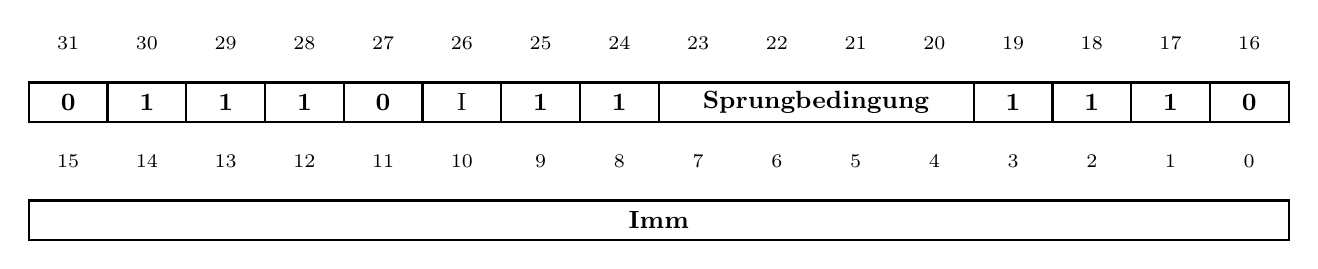
\begin{tikzpicture}
	% Bitnummern oben
	\foreach \x in {0,...,15}
		\pgfmathsetmacro{\number}{int(abs(\x-15)+16)}
		\node at (\x - 0.5, 20.5) {\scriptsize \number};
	% Bitbeschreibungen
	\filldraw[thick, draw=black, fill={rgb:white,255}] (-1, 20) rectangle (0,
	19.5);
	\node (mode) at (-0.5, 19.75) {\small \textbf{0}};
	\filldraw[thick, draw=black, fill={rgb:white,255}] (0, 20) rectangle (1,
	19.5);
	\node (mode) at (0.5, 19.75) {\small \textbf{1}};
	\filldraw[thick, draw=black, fill={rgb:white,255}] (1, 20) rectangle (2,
	19.5);
	\node (mode) at (1.5, 19.75) {\small \textbf{1}};
	\filldraw[thick, draw=black, fill={rgb:white,255}] (2, 20) rectangle (3,
	19.5);
	\node (mode) at (2.5, 19.75) {\small \textbf{1}};
	\filldraw[thick, draw=black, fill={rgb:white,255}] (3, 20) rectangle (4,
	19.5);
	\node (mode) at (3.5, 19.75) {\small \textbf{0}};
	\filldraw[thick, draw=black, fill={rgb:white,255}] (4, 20) rectangle (5,
	19.5);
	\node (mode) at (4.5, 19.75) {\small I};
	\filldraw[thick, draw=black, fill={rgb:white,255}] (5, 20) rectangle (6,
	19.5);
	\node (mode) at (5.5, 19.75) {\small \textbf{1}};
	\filldraw[thick, draw=black, fill={rgb:white,255}] (6, 20) rectangle (7,
	19.5);
	\node (mode) at (6.5, 19.75) {\small \textbf{1}};
	\filldraw[thick, draw=black, fill={rgb:white,255}] (7, 20) rectangle (11,
	19.5);
	\node (mode) at (9, 19.75) {\small \textbf{Sprungbedingung}};
	\filldraw[thick, draw=black, fill={rgb:white,255}] (11, 20) rectangle (12,
	19.5);
	\node (mode) at (11.5, 19.75) {\small \textbf{1}};
	\filldraw[thick, draw=black, fill={rgb:white,255}] (12, 20) rectangle (13,
	19.5);
	\node (mode) at (12.5, 19.75) {\small \textbf{1}};
	\filldraw[thick, draw=black, fill={rgb:white,255}] (13, 20) rectangle (14,
	19.5);
	\node (mode) at (13.5, 19.75) {\small \textbf{1}};
	\filldraw[thick, draw=black, fill={rgb:white,255}] (14, 20) rectangle (15,
	19.5);
	\node (mode) at (14.5, 19.75) {\small \textbf{0}};

	% Bitnummern oben
	\foreach \x in {0,...,15}
		\pgfmathsetmacro{\number}{int(abs(\x-15))}
		\node at (\x - 0.5, 19) {\scriptsize \number};
	% Bitbeschreibungen
	\filldraw[thick, draw=black, fill={rgb:white,255}] (-1, 18.5) rectangle (15,
	18);
	\node (mode) at (7, 18.25) {\small \textbf{Imm}};
\end{tikzpicture}

Springe zu Adresse, wenn die \textbf{Sprungbedingung} erfüllt ist. Dafür wird die
\textbf{Sprungbedingung} mit dem Register \textbf{R14} verglichen. Wenn das Bit
\textbf{I} gesetzt ist, wird der Wert der Konstante \textit{Imm} als Adresse
übernommen (1), andernfalls wird der Wert zum derzeitigen Wert des PC's addiert
(2). Dabei wird im zweiten Fall immer von vorzeichenbehafteten Zahlen
ausgegangen, damit auch Sprünge rückwarts stattfinden können. Weitere
Informationen zur \textbf{Sprungbedingung} sind der
Tabelle~\ref{tab:sprungbedingung} zu entnehmen.

(1) \textit{PC = Imm (wenn Sprungbedingung erfüllt ist)}

(2) \textit{PC = PC + Imm (wenn Sprungbedingung erfüllt ist)}
\section*{mul}
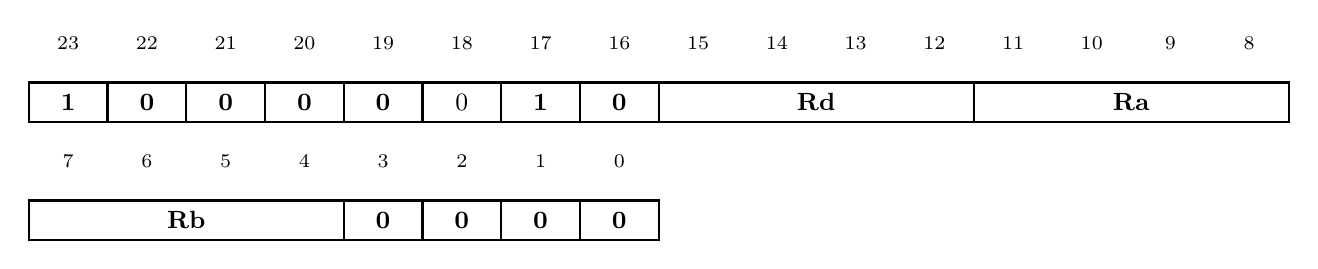
\begin{tikzpicture}
	% Bitnummern oben
	\foreach \x in {0,...,15}
		\pgfmathsetmacro{\number}{int(abs(\x-15)+8)}
		\node at (\x - 0.5, 20.5) {\scriptsize \number};
	% Bitbeschreibungen
	\filldraw[thick, draw=black, fill={rgb:white,255}] (-1, 20) rectangle (0,
	19.5);
	\node (mode) at (-0.5, 19.75) {\small \textbf{1}};
	\filldraw[thick, draw=black, fill={rgb:white,255}] (0, 20) rectangle (1,
	19.5);
	\node (mode) at (0.5, 19.75) {\small \textbf{0}};
	\filldraw[thick, draw=black, fill={rgb:white,255}] (1, 20) rectangle (2,
	19.5);
	\node (mode) at (1.5, 19.75) {\small \textbf{0}};
	\filldraw[thick, draw=black, fill={rgb:white,255}] (2, 20) rectangle (3,
	19.5);
	\node (mode) at (2.5, 19.75) {\small \textbf{0}};
	\filldraw[thick, draw=black, fill={rgb:white,255}] (3, 20) rectangle (4,
	19.5);
	\node (mode) at (3.5, 19.75) {\small \textbf{0}};
	\filldraw[thick, draw=black, fill={rgb:white,255}] (4, 20) rectangle (5,
	19.5);
	\node (mode) at (4.5, 19.75) {\small 0};
	\filldraw[thick, draw=black, fill={rgb:white,255}] (5, 20) rectangle (6,
	19.5);
	\node (mode) at (5.5, 19.75) {\small \textbf{1}};
	\filldraw[thick, draw=black, fill={rgb:white,255}] (6, 20) rectangle (7,
	19.5);
	\node (mode) at (6.5, 19.75) {\small \textbf{0}};
	\filldraw[thick, draw=black, fill={rgb:white,255}] (7, 20) rectangle (11,
	19.5);
	\node (mode) at (9, 19.75) {\small \textbf{Rd}};
	\filldraw[thick, draw=black, fill={rgb:white,255}] (11, 20) rectangle (15,
	19.5);
	\node (mode) at (13, 19.75) {\small \textbf{Ra}};

	% Bitnummern oben
	\foreach \x in {0,...,7}
		\pgfmathsetmacro{\number}{int(abs(\x-7))}
		\node at (\x - 0.5, 19) {\scriptsize \number};
	% Bitbeschreibungen
	\filldraw[thick, draw=black, fill={rgb:white,255}] (-1, 18.5) rectangle (3,
	18);
	\node (mode) at (1, 18.25) {\small \textbf{Rb}};
	\filldraw[thick, draw=black, fill={rgb:white,255}] (3, 18.5) rectangle (4,
	18);
	\node (mode) at (3.5, 18.25) {\small \textbf{0}};
	\filldraw[thick, draw=black, fill={rgb:white,255}] (4, 18.5) rectangle (5,
	18);
	\node (mode) at (4.5, 18.25) {\small \textbf{0}};
	\filldraw[thick, draw=black, fill={rgb:white,255}] (5, 18.5) rectangle (6,
	18);
	\node (mode) at (5.5, 18.25) {\small \textbf{0}};
	\filldraw[thick, draw=black, fill={rgb:white,255}] (6, 18.5) rectangle (7,
	18);
	\node (mode) at (6.5, 18.25) {\small \textbf{0}};
\end{tikzpicture}

Zwei Register werden miteinander multipliziert in das Ergebnis in ein drittes
Register geschrieben.

\textit{Regs[Rd] = Regs[Ra] $\cdot$ Regs[Rb]}
\section*{push}
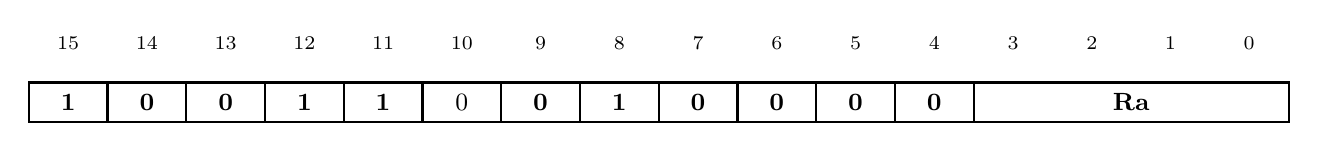
\begin{tikzpicture}
	% Bitnummern oben
	\foreach \x in {0,...,15}
		\pgfmathsetmacro{\number}{int(abs(\x-15))}
		\node at (\x - 0.5, 20.5) {\scriptsize \number};
	% Bitbeschreibungen
	\filldraw[thick, draw=black, fill={rgb:white,255}] (-1, 20) rectangle (0,
	19.5);
	\node (mode) at (-0.5, 19.75) {\small \textbf{1}};
	\filldraw[thick, draw=black, fill={rgb:white,255}] (0, 20) rectangle (1,
	19.5);
	\node (mode) at (0.5, 19.75) {\small \textbf{0}};
	\filldraw[thick, draw=black, fill={rgb:white,255}] (1, 20) rectangle (2,
	19.5);
	\node (mode) at (1.5, 19.75) {\small \textbf{0}};
	\filldraw[thick, draw=black, fill={rgb:white,255}] (2, 20) rectangle (3,
	19.5);
	\node (mode) at (2.5, 19.75) {\small \textbf{1}};
	\filldraw[thick, draw=black, fill={rgb:white,255}] (3, 20) rectangle (4,
	19.5);
	\node (mode) at (3.5, 19.75) {\small \textbf{1}};
	\filldraw[thick, draw=black, fill={rgb:white,255}] (4, 20) rectangle (5,
	19.5);
	\node (mode) at (4.5, 19.75) {\small 0};
	\filldraw[thick, draw=black, fill={rgb:white,255}] (5, 20) rectangle (6,
	19.5);
	\node (mode) at (5.5, 19.75) {\small \textbf{0}};
	\filldraw[thick, draw=black, fill={rgb:white,255}] (6, 20) rectangle (7,
	19.5);
	\node (mode) at (6.5, 19.75) {\small \textbf{1}};
	\filldraw[thick, draw=black, fill={rgb:white,255}] (7, 20) rectangle (8,
	19.5);
	\node (mode) at (7.5, 19.75) {\small \textbf{0}};
	\filldraw[thick, draw=black, fill={rgb:white,255}] (8, 20) rectangle (9,
	19.5);
	\node (mode) at (8.5, 19.75) {\small \textbf{0}};
	\filldraw[thick, draw=black, fill={rgb:white,255}] (9, 20) rectangle (10,
	19.5);
	\node (mode) at (9.5, 19.75) {\small \textbf{0}};
	\filldraw[thick, draw=black, fill={rgb:white,255}] (10, 20) rectangle (11,
	19.5);
	\node (mode) at (10.5, 19.75) {\small \textbf{0}};
	\filldraw[thick, draw=black, fill={rgb:white,255}] (11, 20) rectangle (15,
	19.5);
	\node (mode) at (13, 19.75) {\small \textbf{Ra}};
\end{tikzpicture}

Schiebe den Wert des Registers \textit{Ra} auf den Stack (Stapel).
\section*{pop}
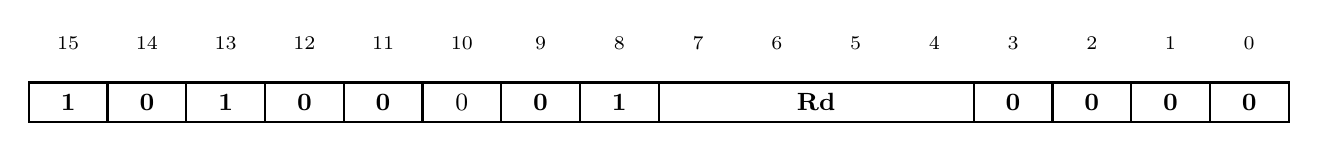
\begin{tikzpicture}
	% Bitnummern oben
	\foreach \x in {0,...,15}
		\pgfmathsetmacro{\number}{int(abs(\x-15))}
		\node at (\x - 0.5, 20.5) {\scriptsize \number};
	% Bitbeschreibungen
	\filldraw[thick, draw=black, fill={rgb:white,255}] (-1, 20) rectangle (0,
	19.5);
	\node (mode) at (-0.5, 19.75) {\small \textbf{1}};
	\filldraw[thick, draw=black, fill={rgb:white,255}] (0, 20) rectangle (1,
	19.5);
	\node (mode) at (0.5, 19.75) {\small \textbf{0}};
	\filldraw[thick, draw=black, fill={rgb:white,255}] (1, 20) rectangle (2,
	19.5);
	\node (mode) at (1.5, 19.75) {\small \textbf{1}};
	\filldraw[thick, draw=black, fill={rgb:white,255}] (2, 20) rectangle (3,
	19.5);
	\node (mode) at (2.5, 19.75) {\small \textbf{0}};
	\filldraw[thick, draw=black, fill={rgb:white,255}] (3, 20) rectangle (4,
	19.5);
	\node (mode) at (3.5, 19.75) {\small \textbf{0}};
	\filldraw[thick, draw=black, fill={rgb:white,255}] (4, 20) rectangle (5,
	19.5);
	\node (mode) at (4.5, 19.75) {\small 0};
	\filldraw[thick, draw=black, fill={rgb:white,255}] (5, 20) rectangle (6,
	19.5);
	\node (mode) at (5.5, 19.75) {\small \textbf{0}};
	\filldraw[thick, draw=black, fill={rgb:white,255}] (6, 20) rectangle (7,
	19.5);
	\node (mode) at (6.5, 19.75) {\small \textbf{1}};
	\filldraw[thick, draw=black, fill={rgb:white,255}] (7, 20) rectangle (11,
	19.5);
	\node (mode) at (9, 19.75) {\small \textbf{Rd}};
	\filldraw[thick, draw=black, fill={rgb:white,255}] (11, 20) rectangle (12,
	19.5);
	\node (mode) at (11.5, 19.75) {\small \textbf{0}};
	\filldraw[thick, draw=black, fill={rgb:white,255}] (12, 20) rectangle (13,
	19.5);
	\node (mode) at (12.5, 19.75) {\small \textbf{0}};
	\filldraw[thick, draw=black, fill={rgb:white,255}] (13, 20) rectangle (14,
	19.5);
	\node (mode) at (13.5, 19.75) {\small \textbf{0}};
	\filldraw[thick, draw=black, fill={rgb:white,255}] (14, 20) rectangle (15,
	19.5);
	\node (mode) at (14.5, 19.75) {\small \textbf{0}};
\end{tikzpicture}

Hole das oberste Element des Stacks und schreibe es in das Register \textit{Rd}.
\section*{call.r}
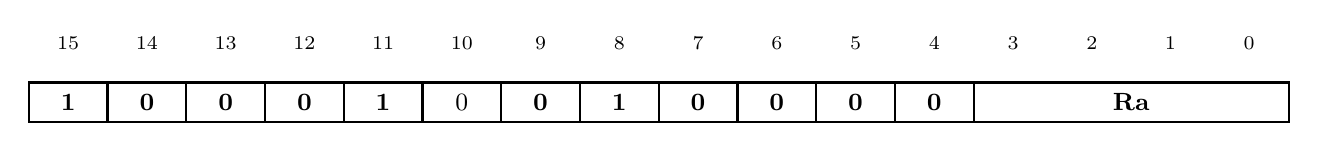
\begin{tikzpicture}
	% Bitnummern oben
	\foreach \x in {0,...,15}
		\pgfmathsetmacro{\number}{int(abs(\x-15))}
		\node at (\x - 0.5, 20.5) {\scriptsize \number};
	% Bitbeschreibungen
	\filldraw[thick, draw=black, fill={rgb:white,255}] (-1, 20) rectangle (0,
	19.5);
	\node (mode) at (-0.5, 19.75) {\small \textbf{1}};
	\filldraw[thick, draw=black, fill={rgb:white,255}] (0, 20) rectangle (1,
	19.5);
	\node (mode) at (0.5, 19.75) {\small \textbf{0}};
	\filldraw[thick, draw=black, fill={rgb:white,255}] (1, 20) rectangle (2,
	19.5);
	\node (mode) at (1.5, 19.75) {\small \textbf{0}};
	\filldraw[thick, draw=black, fill={rgb:white,255}] (2, 20) rectangle (3,
	19.5);
	\node (mode) at (2.5, 19.75) {\small \textbf{0}};
	\filldraw[thick, draw=black, fill={rgb:white,255}] (3, 20) rectangle (4,
	19.5);
	\node (mode) at (3.5, 19.75) {\small \textbf{1}};
	\filldraw[thick, draw=black, fill={rgb:white,255}] (4, 20) rectangle (5,
	19.5);
	\node (mode) at (4.5, 19.75) {\small 0};
	\filldraw[thick, draw=black, fill={rgb:white,255}] (5, 20) rectangle (6,
	19.5);
	\node (mode) at (5.5, 19.75) {\small \textbf{0}};
	\filldraw[thick, draw=black, fill={rgb:white,255}] (6, 20) rectangle (7,
	19.5);
	\node (mode) at (6.5, 19.75) {\small \textbf{1}};
	\filldraw[thick, draw=black, fill={rgb:white,255}] (7, 20) rectangle (8,
	19.5);
	\node (mode) at (7.5, 19.75) {\small \textbf{0}};
	\filldraw[thick, draw=black, fill={rgb:white,255}] (8, 20) rectangle (9,
	19.5);
	\node (mode) at (8.5, 19.75) {\small \textbf{0}};
	\filldraw[thick, draw=black, fill={rgb:white,255}] (9, 20) rectangle (10,
	19.5);
	\node (mode) at (9.5, 19.75) {\small \textbf{0}};
	\filldraw[thick, draw=black, fill={rgb:white,255}] (10, 20) rectangle (11,
	19.5);
	\node (mode) at (10.5, 19.75) {\small \textbf{0}};
	\filldraw[thick, draw=black, fill={rgb:white,255}] (11, 20) rectangle (15,
	19.5);
	\node (mode) at (13, 19.75) {\small \textbf{Ra}};
\end{tikzpicture}

Rufe die Funktion an der Adresse \textit{Ra} auf.

\textbf{Hinweis}: Dieser Befehl tut gleichzeitig die Rückkehraddresse auf den
Stack schieben, damit die Funktion wieder ordnungsgemäß zurückkehren kann.
\section*{call.o, call.i}
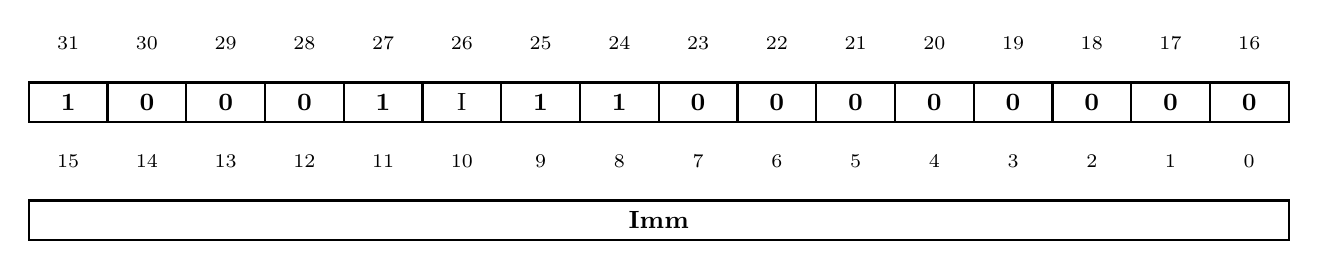
\begin{tikzpicture}
	% Bitnummern oben
	\foreach \x in {0,...,15}
		\pgfmathsetmacro{\number}{int(abs(\x-15)+16)}
		\node at (\x - 0.5, 20.5) {\scriptsize \number};
	% Bitbeschreibungen
	\filldraw[thick, draw=black, fill={rgb:white,255}] (-1, 20) rectangle (0,
	19.5);
	\node (mode) at (-0.5, 19.75) {\small \textbf{1}};
	\filldraw[thick, draw=black, fill={rgb:white,255}] (0, 20) rectangle (1,
	19.5);
	\node (mode) at (0.5, 19.75) {\small \textbf{0}};
	\filldraw[thick, draw=black, fill={rgb:white,255}] (1, 20) rectangle (2,
	19.5);
	\node (mode) at (1.5, 19.75) {\small \textbf{0}};
	\filldraw[thick, draw=black, fill={rgb:white,255}] (2, 20) rectangle (3,
	19.5);
	\node (mode) at (2.5, 19.75) {\small \textbf{0}};
	\filldraw[thick, draw=black, fill={rgb:white,255}] (3, 20) rectangle (4,
	19.5);
	\node (mode) at (3.5, 19.75) {\small \textbf{1}};
	\filldraw[thick, draw=black, fill={rgb:white,255}] (4, 20) rectangle (5,
	19.5);
	\node (mode) at (4.5, 19.75) {\small I};
	\filldraw[thick, draw=black, fill={rgb:white,255}] (5, 20) rectangle (6,
	19.5);
	\node (mode) at (5.5, 19.75) {\small \textbf{1}};
	\filldraw[thick, draw=black, fill={rgb:white,255}] (6, 20) rectangle (7,
	19.5);
	\node (mode) at (6.5, 19.75) {\small \textbf{1}};
	\filldraw[thick, draw=black, fill={rgb:white,255}] (7, 20) rectangle (8,
	19.5);
	\node (mode) at (7.5, 19.75) {\small \textbf{0}};
	\filldraw[thick, draw=black, fill={rgb:white,255}] (8, 20) rectangle (9,
	19.5);
	\node (mode) at (8.5, 19.75) {\small \textbf{0}};
	\filldraw[thick, draw=black, fill={rgb:white,255}] (9, 20) rectangle (10,
	19.5);
	\node (mode) at (9.5, 19.75) {\small \textbf{0}};
	\filldraw[thick, draw=black, fill={rgb:white,255}] (10, 20) rectangle (11,
	19.5);
	\node (mode) at (10.5, 19.75) {\small \textbf{0}};
	\filldraw[thick, draw=black, fill={rgb:white,255}] (11, 20) rectangle (12,
	19.5);
	\node (mode) at (11.5, 19.75) {\small \textbf{0}};
	\filldraw[thick, draw=black, fill={rgb:white,255}] (12, 20) rectangle (13,
	19.5);
	\node (mode) at (12.5, 19.75) {\small \textbf{0}};
	\filldraw[thick, draw=black, fill={rgb:white,255}] (13, 20) rectangle (14,
	19.5);
	\node (mode) at (13.5, 19.75) {\small \textbf{0}};
	\filldraw[thick, draw=black, fill={rgb:white,255}] (14, 20) rectangle (15,
	19.5);
	\node (mode) at (14.5, 19.75) {\small \textbf{0}};

	% Bitnummern oben
	\foreach \x in {0,...,15}
		\pgfmathsetmacro{\number}{int(abs(\x-15))}
		\node at (\x - 0.5, 19) {\scriptsize \number};
	% Bitbeschreibungen
	\filldraw[thick, draw=black, fill={rgb:white,255}] (-1, 18.5) rectangle (15,
	18);
	\node (mode) at (7, 18.25) {\small \textbf{Imm}};
\end{tikzpicture}

Rufe die Funktion an der Adresse \textit{Ra} auf. Wenn das Bit \textbf{I}
gesetzt ist, wird der Wert der Konstante \textit{Imm} als Adresse übernommen
(1), andernfalls wird der Wert zum derzeitigen Wert des PC's addiert (2).

(1) \textit{PC = Imm (wenn Sprungbedingung erfüllt ist)}

(2) \textit{PC = PC + Imm (wenn Sprungbedingung erfüllt ist)}

\textbf{Hinweis}: Dieser Befehl tut gleichzeitig die Rückkehraddresse auf den
Stack schieben, damit die Funktion wieder ordnungsgemäß zurückkehren kann.
\section*{ret}
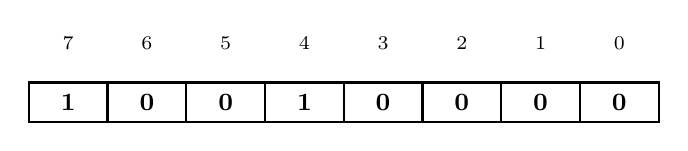
\begin{tikzpicture}
	% Bitnummern oben
	\foreach \x in {0,...,7}
		\pgfmathsetmacro{\number}{int(abs(\x-7))}
		\node at (\x - 0.5, 20.5) {\scriptsize \number};
	% Bitbeschreibungen
	\filldraw[thick, draw=black, fill={rgb:white,255}] (-1, 20) rectangle (0,
	19.5);
	\node (mode) at (-0.5, 19.75) {\small \textbf{1}};
	\filldraw[thick, draw=black, fill={rgb:white,255}] (0, 20) rectangle (1,
	19.5);
	\node (mode) at (0.5, 19.75) {\small \textbf{0}};
	\filldraw[thick, draw=black, fill={rgb:white,255}] (1, 20) rectangle (2,
	19.5);
	\node (mode) at (1.5, 19.75) {\small \textbf{0}};
	\filldraw[thick, draw=black, fill={rgb:white,255}] (2, 20) rectangle (3,
	19.5);
	\node (mode) at (2.5, 19.75) {\small \textbf{1}};
	\filldraw[thick, draw=black, fill={rgb:white,255}] (3, 20) rectangle (4,
	19.5);
	\node (mode) at (3.5, 19.75) {\small \textbf{0}};
	\filldraw[thick, draw=black, fill={rgb:white,255}] (4, 20) rectangle (5,
	19.5);
	\node (mode) at (4.5, 19.75) {\small \textbf{0}};
	\filldraw[thick, draw=black, fill={rgb:white,255}] (5, 20) rectangle (6,
	19.5);
	\node (mode) at (5.5, 19.75) {\small \textbf{0}};
	\filldraw[thick, draw=black, fill={rgb:white,255}] (6, 20) rectangle (7,
	19.5);
	\node (mode) at (6.5, 19.75) {\small \textbf{0}};
\end{tikzpicture}

Beendet die Funktion und kehrt damit zurück zum Aufruf der Funktion. Die
Rückkehraddresse wird aus dem Stack entnommen.
\section*{test.r}
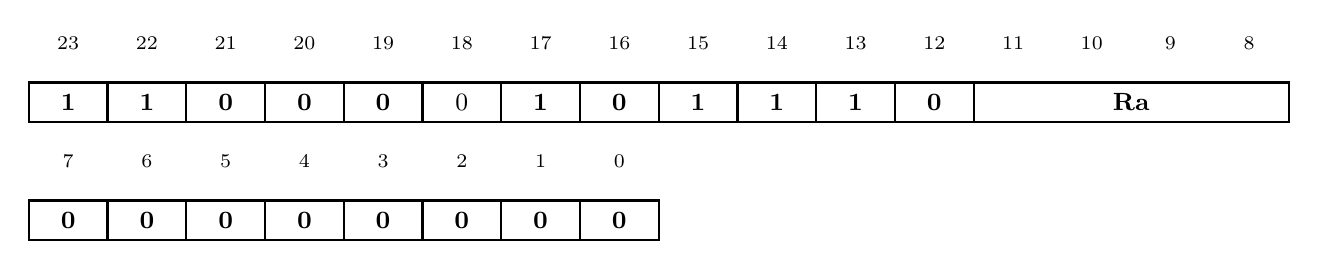
\begin{tikzpicture}
	% Bitnummern oben
	\foreach \x in {0,...,15}
		\pgfmathsetmacro{\number}{int(abs(\x-15)+8)}
		\node at (\x - 0.5, 20.5) {\scriptsize \number};
	% Bitbeschreibungen
	\filldraw[thick, draw=black, fill={rgb:white,255}] (-1, 20) rectangle (0,
	19.5);
	\node (mode) at (-0.5, 19.75) {\small \textbf{1}};
	\filldraw[thick, draw=black, fill={rgb:white,255}] (0, 20) rectangle (1,
	19.5);
	\node (mode) at (0.5, 19.75) {\small \textbf{1}};
	\filldraw[thick, draw=black, fill={rgb:white,255}] (1, 20) rectangle (2,
	19.5);
	\node (mode) at (1.5, 19.75) {\small \textbf{0}};
	\filldraw[thick, draw=black, fill={rgb:white,255}] (2, 20) rectangle (3,
	19.5);
	\node (mode) at (2.5, 19.75) {\small \textbf{0}};
	\filldraw[thick, draw=black, fill={rgb:white,255}] (3, 20) rectangle (4,
	19.5);
	\node (mode) at (3.5, 19.75) {\small \textbf{0}};
	\filldraw[thick, draw=black, fill={rgb:white,255}] (4, 20) rectangle (5,
	19.5);
	\node (mode) at (4.5, 19.75) {\small 0};
	\filldraw[thick, draw=black, fill={rgb:white,255}] (5, 20) rectangle (6,
	19.5);
	\node (mode) at (5.5, 19.75) {\small \textbf{1}};
	\filldraw[thick, draw=black, fill={rgb:white,255}] (6, 20) rectangle (7,
	19.5);
	\node (mode) at (6.5, 19.75) {\small \textbf{0}};
	\filldraw[thick, draw=black, fill={rgb:white,255}] (7, 20) rectangle (8,
	19.5);
	\node (mode) at (7.5, 19.75) {\small \textbf{1}};
	\filldraw[thick, draw=black, fill={rgb:white,255}] (8, 20) rectangle (9,
	19.5);
	\node (mode) at (8.5, 19.75) {\small \textbf{1}};
	\filldraw[thick, draw=black, fill={rgb:white,255}] (9, 20) rectangle (10,
	19.5);
	\node (mode) at (9.5, 19.75) {\small \textbf{1}};
	\filldraw[thick, draw=black, fill={rgb:white,255}] (10, 20) rectangle (11,
	19.5);
	\node (mode) at (10.5, 19.75) {\small \textbf{0}};
	\filldraw[thick, draw=black, fill={rgb:white,255}] (11, 20) rectangle (15,
	19.5);
	\node (mode) at (13, 19.75) {\small \textbf{Ra}};

	% Bitnummern oben
	\foreach \x in {0,...,7}
		\pgfmathsetmacro{\number}{int(abs(\x-7))}
		\node at (\x - 0.5, 19) {\scriptsize \number};
	% Bitbeschreibungen
	\filldraw[thick, draw=black, fill={rgb:white,255}] (-1, 18.5) rectangle (0,
	18);
	\node (mode) at (-0.5, 18.25) {\small \textbf{0}};
	\filldraw[thick, draw=black, fill={rgb:white,255}] (0, 18.5) rectangle (1,
	18);
	\node (mode) at (0.5, 18.25) {\small \textbf{0}};
	\filldraw[thick, draw=black, fill={rgb:white,255}] (1, 18.5) rectangle (2,
	18);
	\node (mode) at (1.5, 18.25) {\small \textbf{0}};
	\filldraw[thick, draw=black, fill={rgb:white,255}] (2, 18.5) rectangle (3,
	18);
	\node (mode) at (2.5, 18.25) {\small \textbf{0}};
	\filldraw[thick, draw=black, fill={rgb:white,255}] (3, 18.5) rectangle (4,
	18);
	\node (mode) at (3.5, 18.25) {\small \textbf{0}};
	\filldraw[thick, draw=black, fill={rgb:white,255}] (4, 18.5) rectangle (5,
	18);
	\node (mode) at (4.5, 18.25) {\small \textbf{0}};
	\filldraw[thick, draw=black, fill={rgb:white,255}] (5, 18.5) rectangle (6,
	18);
	\node (mode) at (5.5, 18.25) {\small \textbf{0}};
	\filldraw[thick, draw=black, fill={rgb:white,255}] (6, 18.5) rectangle (7,
	18);
	\node (mode) at (6.5, 18.25) {\small \textbf{0}};
\end{tikzpicture}

Teste das Register \textit{Ra} auf besondere Eigenschaften und schreibe das
Ergebnis als \textbf{Testbitmaske} in das Register \textbf{R14}.

\textit{Regs[14] = test(Regs[Ra])}
\section*{test.b}
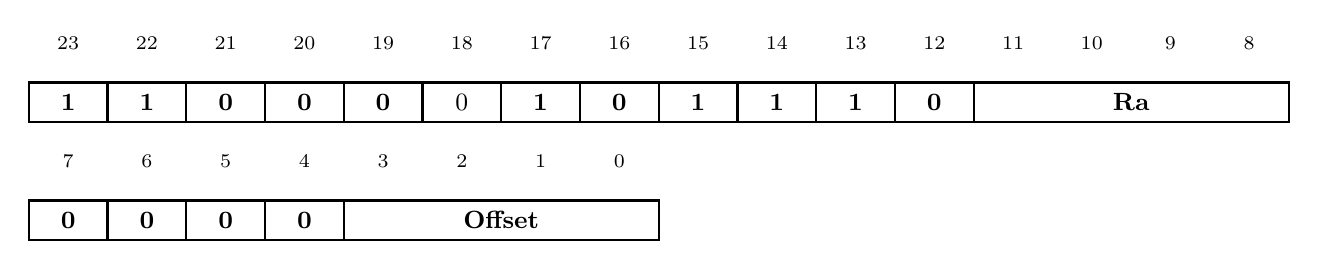
\begin{tikzpicture}
	% Bitnummern oben
	\foreach \x in {0,...,15}
		\pgfmathsetmacro{\number}{int(abs(\x-15)+8)}
		\node at (\x - 0.5, 20.5) {\scriptsize \number};
	% Bitbeschreibungen
	\filldraw[thick, draw=black, fill={rgb:white,255}] (-1, 20) rectangle (0,
	19.5);
	\node (mode) at (-0.5, 19.75) {\small \textbf{1}};
	\filldraw[thick, draw=black, fill={rgb:white,255}] (0, 20) rectangle (1,
	19.5);
	\node (mode) at (0.5, 19.75) {\small \textbf{1}};
	\filldraw[thick, draw=black, fill={rgb:white,255}] (1, 20) rectangle (2,
	19.5);
	\node (mode) at (1.5, 19.75) {\small \textbf{0}};
	\filldraw[thick, draw=black, fill={rgb:white,255}] (2, 20) rectangle (3,
	19.5);
	\node (mode) at (2.5, 19.75) {\small \textbf{0}};
	\filldraw[thick, draw=black, fill={rgb:white,255}] (3, 20) rectangle (4,
	19.5);
	\node (mode) at (3.5, 19.75) {\small \textbf{0}};
	\filldraw[thick, draw=black, fill={rgb:white,255}] (4, 20) rectangle (5,
	19.5);
	\node (mode) at (4.5, 19.75) {\small 0};
	\filldraw[thick, draw=black, fill={rgb:white,255}] (5, 20) rectangle (6,
	19.5);
	\node (mode) at (5.5, 19.75) {\small \textbf{1}};
	\filldraw[thick, draw=black, fill={rgb:white,255}] (6, 20) rectangle (7,
	19.5);
	\node (mode) at (6.5, 19.75) {\small \textbf{0}};
	\filldraw[thick, draw=black, fill={rgb:white,255}] (7, 20) rectangle (8,
	19.5);
	\node (mode) at (7.5, 19.75) {\small \textbf{1}};
	\filldraw[thick, draw=black, fill={rgb:white,255}] (8, 20) rectangle (9,
	19.5);
	\node (mode) at (8.5, 19.75) {\small \textbf{1}};
	\filldraw[thick, draw=black, fill={rgb:white,255}] (9, 20) rectangle (10,
	19.5);
	\node (mode) at (9.5, 19.75) {\small \textbf{1}};
	\filldraw[thick, draw=black, fill={rgb:white,255}] (10, 20) rectangle (11,
	19.5);
	\node (mode) at (10.5, 19.75) {\small \textbf{0}};
	\filldraw[thick, draw=black, fill={rgb:white,255}] (11, 20) rectangle (15,
	19.5);
	\node (mode) at (13, 19.75) {\small \textbf{Ra}};

	% Bitnummern oben
	\foreach \x in {0,...,7}
		\pgfmathsetmacro{\number}{int(abs(\x-7))}
		\node at (\x - 0.5, 19) {\scriptsize \number};
	% Bitbeschreibungen
	\filldraw[thick, draw=black, fill={rgb:white,255}] (-1, 18.5) rectangle (0,
	18);
	\node (mode) at (-0.5, 18.25) {\small \textbf{0}};
	\filldraw[thick, draw=black, fill={rgb:white,255}] (0, 18.5) rectangle (1,
	18);
	\node (mode) at (0.5, 18.25) {\small \textbf{0}};
	\filldraw[thick, draw=black, fill={rgb:white,255}] (1, 18.5) rectangle (2,
	18);
	\node (mode) at (1.5, 18.25) {\small \textbf{0}};
	\filldraw[thick, draw=black, fill={rgb:white,255}] (2, 18.5) rectangle (3,
	18);
	\node (mode) at (2.5, 18.25) {\small \textbf{0}};
	\filldraw[thick, draw=black, fill={rgb:white,255}] (3, 18.5) rectangle (7,
	18);
	\node (mode) at (5, 18.25) {\small \textbf{Offset}};
\end{tikzpicture}

Teste ein Bit des Registers \textit{Ra}. Die Eigenschaften werden mit der
\textbf{Testbitmaske} festgehalten und in das Register \textbf{R14} geschrieben.

\textit{Regs[14] = test(Regs[Ra<Offset>])}
\subsubsection*{Testbitmaske}
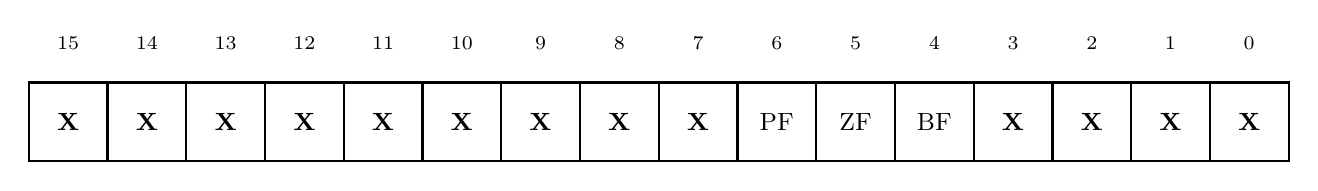
\begin{tikzpicture}
	% Bitnummern oben
	\foreach \x in {0,...,15}
		\pgfmathsetmacro{\number}{int(abs(\x-15))}
		\node at (\x - 0.5, 20.5) {\scriptsize \number};
	% Bitbeschreibungen
	\filldraw[thick, draw=black, fill={rgb:white,255}] (-1, 20) rectangle (0,
	19);
	\node (mode) at (-0.5, 19.5) {\small \textbf{X}};
	\filldraw[thick, draw=black, fill={rgb:white,255}] (0, 20) rectangle (1,
	19);
	\node (mode) at (0.5, 19.5) {\small \textbf{X}};
	\filldraw[thick, draw=black, fill={rgb:white,255}] (1, 20) rectangle (2,
	19);
	\node (mode) at (1.5, 19.5) {\small \textbf{X}};
	\filldraw[thick, draw=black, fill={rgb:white,255}] (2, 20) rectangle (3,
	19);
	\node (mode) at (2.5, 19.5) {\small \textbf{X}};
	\filldraw[thick, draw=black, fill={rgb:white,255}] (3, 20) rectangle (4,
	19);
	\node (mode) at (3.5, 19.5) {\small \textbf{X}};
	\filldraw[thick, draw=black, fill={rgb:white,255}] (4, 20) rectangle (5,
	19);
	\node (mode) at (4.5, 19.5) {\small \textbf{X}};
	\filldraw[thick, draw=black, fill={rgb:white,255}] (5, 20) rectangle (6,
	19);
	\node (mode) at (5.5, 19.5) {\small \textbf{X}};
	\filldraw[thick, draw=black, fill={rgb:white,255}] (6, 20) rectangle (7,
	19);
	\node (mode) at (6.5, 19.5) {\small \textbf{X}};
	\filldraw[thick, draw=black, fill={rgb:white,255}] (7, 20) rectangle (8,
	19);
	\node (mode) at (7.5, 19.5) {\small \textbf{X}};
	\filldraw[thick, draw=black, fill={rgb:white,255}] (8, 20) rectangle (9,
	19);
	\node (mode) at (8.5, 19.5) {\small PF};
	\filldraw[thick, draw=black, fill={rgb:white,255}] (9, 20) rectangle (10,
	19);
	\node (mode) at (9.5, 19.5) {\small ZF};
	\filldraw[thick, draw=black, fill={rgb:white,255}] (10, 20) rectangle (11,
	19);
	\node (mode) at (10.5, 19.5) {\small BF};
	\filldraw[thick, draw=black, fill={rgb:white,255}] (11, 20) rectangle (12,
	19);
	\node (mode) at (11.5, 19.5) {\small \textbf{X}};
	\filldraw[thick, draw=black, fill={rgb:white,255}] (12, 20) rectangle (13,
	19);
	\node (mode) at (12.5, 19.5) {\small \textbf{X}};
	\filldraw[thick, draw=black, fill={rgb:white,255}] (13, 20) rectangle (14,
	19);
	\node (mode) at (13.5, 19.5) {\small \textbf{X}};
	\filldraw[thick, draw=black, fill={rgb:white,255}] (14, 20) rectangle (15,
	19);
	\node (mode) at (14.5, 19.5) {\small \textbf{X}};
\end{tikzpicture}


\textbf{PF}: Paritätsbit (gerade Parität)

\textbf{ZF}: A == 0

\textbf{BF}: Bit null (für \textit{test.b})
\section*{hlt}
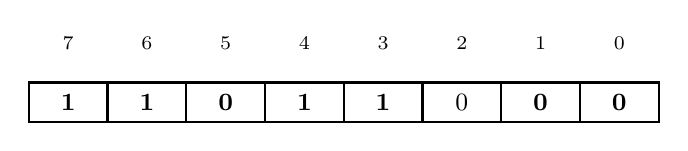
\begin{tikzpicture}
	% Bitnummern oben
	\foreach \x in {0,...,7}
		\pgfmathsetmacro{\number}{int(abs(\x-7))}
		\node at (\x - 0.5, 20.5) {\scriptsize \number};
	% Bitbeschreibungen
	\filldraw[thick, draw=black, fill={rgb:white,255}] (-1, 20) rectangle (0,
	19.5);
	\node (mode) at (-0.5, 19.75) {\small \textbf{1}};
	\filldraw[thick, draw=black, fill={rgb:white,255}] (0, 20) rectangle (1,
	19.5);
	\node (mode) at (0.5, 19.75) {\small \textbf{1}};
	\filldraw[thick, draw=black, fill={rgb:white,255}] (1, 20) rectangle (2,
	19.5);
	\node (mode) at (1.5, 19.75) {\small \textbf{0}};
	\filldraw[thick, draw=black, fill={rgb:white,255}] (2, 20) rectangle (3,
	19.5);
	\node (mode) at (2.5, 19.75) {\small \textbf{1}};
	\filldraw[thick, draw=black, fill={rgb:white,255}] (3, 20) rectangle (4,
	19.5);
	\node (mode) at (3.5, 19.75) {\small \textbf{1}};
	\filldraw[thick, draw=black, fill={rgb:white,255}] (4, 20) rectangle (5,
	19.5);
	\node (mode) at (4.5, 19.75) {\small 0};
	\filldraw[thick, draw=black, fill={rgb:white,255}] (5, 20) rectangle (6,
	19.5);
	\node (mode) at (5.5, 19.75) {\small \textbf{0}};
	\filldraw[thick, draw=black, fill={rgb:white,255}] (6, 20) rectangle (7,
	19.5);
	\node (mode) at (6.5, 19.75) {\small \textbf{0}};
\end{tikzpicture}

Stoppt die CPU. Keine weiteren Befehle werden ausgeführt.
\clearpage
\section*{set}
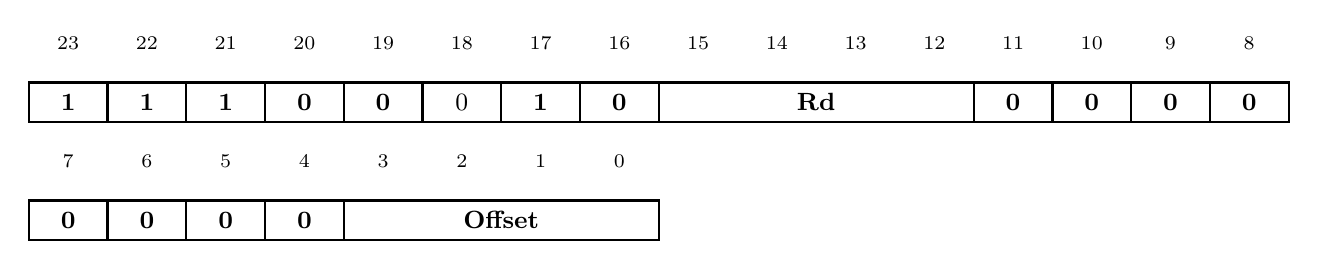
\begin{tikzpicture}
	% Bitnummern oben
	\foreach \x in {0,...,15}
		\pgfmathsetmacro{\number}{int(abs(\x-15)+8)}
		\node at (\x - 0.5, 20.5) {\scriptsize \number};
	% Bitbeschreibungen
	\filldraw[thick, draw=black, fill={rgb:white,255}] (-1, 20) rectangle (0,
	19.5);
	\node (mode) at (-0.5, 19.75) {\small \textbf{1}};
	\filldraw[thick, draw=black, fill={rgb:white,255}] (0, 20) rectangle (1,
	19.5);
	\node (mode) at (0.5, 19.75) {\small \textbf{1}};
	\filldraw[thick, draw=black, fill={rgb:white,255}] (1, 20) rectangle (2,
	19.5);
	\node (mode) at (1.5, 19.75) {\small \textbf{1}};
	\filldraw[thick, draw=black, fill={rgb:white,255}] (2, 20) rectangle (3,
	19.5);
	\node (mode) at (2.5, 19.75) {\small \textbf{0}};
	\filldraw[thick, draw=black, fill={rgb:white,255}] (3, 20) rectangle (4,
	19.5);
	\node (mode) at (3.5, 19.75) {\small \textbf{0}};
	\filldraw[thick, draw=black, fill={rgb:white,255}] (4, 20) rectangle (5,
	19.5);
	\node (mode) at (4.5, 19.75) {\small 0};
	\filldraw[thick, draw=black, fill={rgb:white,255}] (5, 20) rectangle (6,
	19.5);
	\node (mode) at (5.5, 19.75) {\small \textbf{1}};
	\filldraw[thick, draw=black, fill={rgb:white,255}] (6, 20) rectangle (7,
	19.5);
	\node (mode) at (6.5, 19.75) {\small \textbf{0}};
	\filldraw[thick, draw=black, fill={rgb:white,255}] (7, 20) rectangle (11,
	19.5);
	\node (mode) at (9, 19.75) {\small \textbf{Rd}};
	\filldraw[thick, draw=black, fill={rgb:white,255}] (11, 20) rectangle (12,
	19.5);
	\node (mode) at (11.5, 19.75) {\small \textbf{0}};
	\filldraw[thick, draw=black, fill={rgb:white,255}] (12, 20) rectangle (13,
	19.5);
	\node (mode) at (12.5, 19.75) {\small \textbf{0}};
	\filldraw[thick, draw=black, fill={rgb:white,255}] (13, 20) rectangle (14,
	19.5);
	\node (mode) at (13.5, 19.75) {\small \textbf{0}};
	\filldraw[thick, draw=black, fill={rgb:white,255}] (14, 20) rectangle (15,
	19.5);
	\node (mode) at (14.5, 19.75) {\small \textbf{0}};

	% Bitnummern oben
	\foreach \x in {0,...,7}
		\pgfmathsetmacro{\number}{int(abs(\x-7))}
		\node at (\x - 0.5, 19) {\scriptsize \number};
	% Bitbeschreibungen
	\filldraw[thick, draw=black, fill={rgb:white,255}] (-1, 18.5) rectangle (0,
	18);
	\node (mode) at (-0.5, 18.25) {\small \textbf{0}};
	\filldraw[thick, draw=black, fill={rgb:white,255}] (0, 18.5) rectangle (1,
	18);
	\node (mode) at (0.5, 18.25) {\small \textbf{0}};
	\filldraw[thick, draw=black, fill={rgb:white,255}] (1, 18.5) rectangle (2,
	18);
	\node (mode) at (1.5, 18.25) {\small \textbf{0}};
	\filldraw[thick, draw=black, fill={rgb:white,255}] (2, 18.5) rectangle (3,
	18);
	\node (mode) at (2.5, 18.25) {\small \textbf{0}};
	\filldraw[thick, draw=black, fill={rgb:white,255}] (3, 18.5) rectangle (7,
	18);
	\node (mode) at (5, 18.25) {\small \textbf{Offset}};
\end{tikzpicture}

Setze ein Bit des Registers \textit{Rd} auf den (logischen) Wert 1. Das zu
setzende Bit wird durch den \textbf{Offset} angegeben.

\textit{Regs[Rd<Offset>] = 1}
\section*{clr}
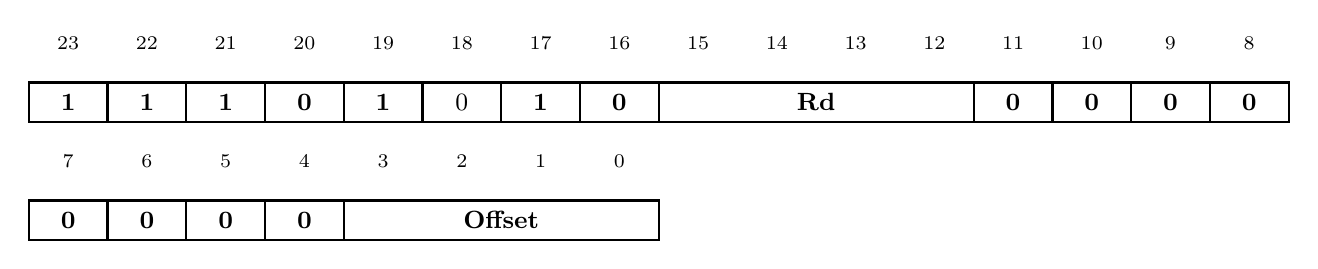
\begin{tikzpicture}
	% Bitnummern oben
	\foreach \x in {0,...,15}
		\pgfmathsetmacro{\number}{int(abs(\x-15)+8)}
		\node at (\x - 0.5, 20.5) {\scriptsize \number};
	% Bitbeschreibungen
	\filldraw[thick, draw=black, fill={rgb:white,255}] (-1, 20) rectangle (0,
	19.5);
	\node (mode) at (-0.5, 19.75) {\small \textbf{1}};
	\filldraw[thick, draw=black, fill={rgb:white,255}] (0, 20) rectangle (1,
	19.5);
	\node (mode) at (0.5, 19.75) {\small \textbf{1}};
	\filldraw[thick, draw=black, fill={rgb:white,255}] (1, 20) rectangle (2,
	19.5);
	\node (mode) at (1.5, 19.75) {\small \textbf{1}};
	\filldraw[thick, draw=black, fill={rgb:white,255}] (2, 20) rectangle (3,
	19.5);
	\node (mode) at (2.5, 19.75) {\small \textbf{0}};
	\filldraw[thick, draw=black, fill={rgb:white,255}] (3, 20) rectangle (4,
	19.5);
	\node (mode) at (3.5, 19.75) {\small \textbf{1}};
	\filldraw[thick, draw=black, fill={rgb:white,255}] (4, 20) rectangle (5,
	19.5);
	\node (mode) at (4.5, 19.75) {\small 0};
	\filldraw[thick, draw=black, fill={rgb:white,255}] (5, 20) rectangle (6,
	19.5);
	\node (mode) at (5.5, 19.75) {\small \textbf{1}};
	\filldraw[thick, draw=black, fill={rgb:white,255}] (6, 20) rectangle (7,
	19.5);
	\node (mode) at (6.5, 19.75) {\small \textbf{0}};
	\filldraw[thick, draw=black, fill={rgb:white,255}] (7, 20) rectangle (11,
	19.5);
	\node (mode) at (9, 19.75) {\small \textbf{Rd}};
	\filldraw[thick, draw=black, fill={rgb:white,255}] (11, 20) rectangle (12,
	19.5);
	\node (mode) at (11.5, 19.75) {\small \textbf{0}};
	\filldraw[thick, draw=black, fill={rgb:white,255}] (12, 20) rectangle (13,
	19.5);
	\node (mode) at (12.5, 19.75) {\small \textbf{0}};
	\filldraw[thick, draw=black, fill={rgb:white,255}] (13, 20) rectangle (14,
	19.5);
	\node (mode) at (13.5, 19.75) {\small \textbf{0}};
	\filldraw[thick, draw=black, fill={rgb:white,255}] (14, 20) rectangle (15,
	19.5);
	\node (mode) at (14.5, 19.75) {\small \textbf{0}};

	% Bitnummern oben
	\foreach \x in {0,...,7}
		\pgfmathsetmacro{\number}{int(abs(\x-7))}
		\node at (\x - 0.5, 19) {\scriptsize \number};
	% Bitbeschreibungen
	\filldraw[thick, draw=black, fill={rgb:white,255}] (-1, 18.5) rectangle (0,
	18);
	\node (mode) at (-0.5, 18.25) {\small \textbf{0}};
	\filldraw[thick, draw=black, fill={rgb:white,255}] (0, 18.5) rectangle (1,
	18);
	\node (mode) at (0.5, 18.25) {\small \textbf{0}};
	\filldraw[thick, draw=black, fill={rgb:white,255}] (1, 18.5) rectangle (2,
	18);
	\node (mode) at (1.5, 18.25) {\small \textbf{0}};
	\filldraw[thick, draw=black, fill={rgb:white,255}] (2, 18.5) rectangle (3,
	18);
	\node (mode) at (2.5, 18.25) {\small \textbf{0}};
	\filldraw[thick, draw=black, fill={rgb:white,255}] (3, 18.5) rectangle (7,
	18);
	\node (mode) at (5, 18.25) {\small \textbf{Offset}};
\end{tikzpicture}

Lösche ein Bit des Registers \textit{Rd}, wodurch das Bit auf den (logischen)
Wert 0 gesetzt wird. Das zu löschende Bit wird durch den \textbf{Offset} angegeben.

\textit{Regs[Rd<Offset>] = 0}
